\documentclass[twoside,11pt,openright]{report}
\usepackage{minted}
\usepackage[utf8]{inputenc}
\usepackage[english]{babel}
\usepackage{a4}
\usepackage{latexsym}
\usepackage{amssymb}
\usepackage{amsmath}
\usepackage{amsthm}
\usepackage{mathpartir}
\usepackage{epsfig}
\usepackage[T1]{fontenc}
\usepackage{stmaryrd}
\usepackage{color}
\usepackage{epstopdf}
\usepackage{microtype}
\usepackage{hyperref}
\usepackage[en-GB]{datetime2}
\DTMlangsetup[en-GB]{showdayofmonth=false}
\usepackage{lipsum}
\usepackage{caption}
\usepackage{subcaption}
\usepackage{iris}
\usepackage{heaplang}
\usepackage{tikz}
\usetikzlibrary{calc,shapes.multipart,chains,arrows}
\usepackage{xspace}
\usepackage{lineno}

\renewcommand*\sfdefault{lmss}
\renewcommand*\ttdefault{txtt}

% Theorems, Corollaries, and Lemmas
\newtheorem{theorem}{Theorem}
\newtheorem{corollary}{Corollary}[theorem]
\newtheorem{lemma}[theorem]{Lemma}

\newtheorem{definition}{Definition}[section]


\newcommand{\isLock}{\operatorname{isLock}}
\newcommand{\locked}{\operatorname{locked}}
\newcommand{\issued}{\operatorname{issued}}
\newcommand{\newLock}{\operatorname{newLock}}
\newcommand{\acquire}{\operatorname{acquire}}
\newcommand{\wait}{\operatorname{wait}}
\newcommand{\release}{\operatorname{release}}
\newcommand{\lockInv}{\operatorname{lockInv}}
\newcommand{\initialise}{\operatorname{initialize}}
\newcommand{\enqueue}{\operatorname{enqueue}}
\newcommand{\dequeue}{\operatorname{dequeue}}

\newcommand{\isqueue}{\operatorname{is\_queue}}
\newcommand{\isqueueseq}{\operatorname{is\_queue\_seq}}
\newcommand{\isqueueconc}{\operatorname{is\_queue\_conc}}

\newcommand{\isLLchain}[1]{\operatorname{isLL\_chain} \; #1}
\newcommand{\isLL}{\operatorname{isLL}}

\newcommand{\locin}[1]{\loc_{#1\_\text{in}}}
\newcommand{\locout}[1]{\loc_{#1\_\text{out}}}

\newcommand{\nIn}[1]{\operatorname{in} \; #1}
\newcommand{\nVal}[1]{\operatorname{val} \; #1}
\newcommand{\nOut}[1]{\operatorname{out} \; #1}

\newcommand{\StaticState}{\textbf{Static}}
\newcommand{\EnqueueState}{\textbf{Enqueue}}
\newcommand{\DequeueState}{\textbf{Dequeue}}
\newcommand{\BothState}{\textbf{Both}}

\newcommand{\Qg}{Q_\gname}
\newcommand{\Qgseq}{Q_{\gname S}}
\newcommand{\Qgconc}{Q_{\gname C}}
\newcommand{\Qghocap}{Q_{\gname H}}

\newcommand{\TokE}[1]{\operatorname{TokE}\ #1}
\newcommand{\TokEQg}{\TokE{\Qg}}
\newcommand{\ToknE}[1]{\operatorname{ToknE}\ #1}
\newcommand{\ToknEQg}{\ToknE{\Qg}}
\newcommand{\TokD}[1]{\operatorname{TokD}\ #1}
\newcommand{\TokDQg}{\TokD{\Qg}}
\newcommand{\ToknD}[1]{\operatorname{ToknD}\ #1}
\newcommand{\ToknDQg}{\ToknD{\Qg}}
\newcommand{\TokBefore}[1]{\operatorname{TokBefore}\ #1}
\newcommand{\TokBeforeQg}{\TokBefore{\Qg}}
\newcommand{\TokAfter}[1]{\operatorname{TokAfter}\ #1}
\newcommand{\TokAfterQg}{\TokBefore{\Qg}}
\newcommand{\TokUpdated}[1]{\operatorname{TokUpdated}\ #1}
\newcommand{\TokUpdatedQg}{\TokUpdated{\Qg}}

\newcommand\catenate{\mathbin{\text{\ttfamily\upshape ++}}}

\newcommand{\BB}{\ensuremath{\mathbb{B}}}
\newcommand{\Cc}{\ensuremath{\mathbf{C}}}
\newcommand{\El}{\ensuremath{\mathcal{E}}}
\newcommand{\Sl}{\ensuremath{\mathcal{S}}}
\newcommand{\Ul}{\ensuremath{\mathcal{U}}}
\newcommand{\Dl}{\ensuremath{\mathcal{D}}}
\newcommand{\Fl}{\ensuremath{\mathcal{F}}}
\newcommand{\Pl}{\ensuremath{\mathcal{P}}}
\newcommand{\Tl}{\ensuremath{\mathcal{T}}}
\newcommand{\CC}{\ensuremath{\mathbb{C}}}
\newcommand{\KK}{\ensuremath{\mathbb{K}}}
\newcommand{\PP}{\ensuremath{\mathbb{P}}}
\newcommand{\VV}{\ensuremath{\mathbb{V}}}
\newcommand{\UU}{\ensuremath{\mathbb{U}}}
\newcommand{\DD}{\ensuremath{\mathbb{D}}}
\newcommand{\Ml}{\ensuremath{\mathcal{M}}}
\newcommand{\Vl}{\ensuremath{\mathcal{V}}}
\newcommand{\Il}{\ensuremath{\mathcal{I}}}
\newcommand{\Cl}{\ensuremath{\mathcal{C}}}
\newcommand{\Bl}{\ensuremath{\mathcal{B}}}
\newcommand{\Al}{\ensuremath{\mathcal{A}}}
\newcommand{\Gl}{\ensuremath{\mathcal{G}}}
\newcommand{\Nl}{\ensuremath{\mathcal{N}}}
\newcommand{\AAA}{\ensuremath{\mathbb{A}}}
\newcommand{\EE}{\ensuremath{\mathbb{E}}}

\newcommand{\isNode}[1]{\nIn{#1} \mapsto^{\persistently} (\nVal{#1}, \nOut{#1})}

\newcommand{\abstractstatefrac}[3]{#1 \Mapsto\kern-0.5ex\tfrac{1}{#2} #3}
\newcommand{\abstractstate}[3]{#1 \Mapsto^{#2}_{\circ} #3}
\newcommand{\abstractstatefullfrag}[2]{#1 \Mapsto_{\circ} #2}
\newcommand{\abstractstateauth}[2]{#1 \Mapsto_{\bullet} #2}

\newcommand{\reach}[2]{#1 \leadsto #2}
\newcommand{\ar}[2]{#1 \dashrightarrow #2}
\newcommand{\ap}[2]{#1 \rightarrowtail #2}

\newcommand{\todo}[1]{{\color[rgb]{.5,0,0}\textbf{$\blacktriangleright$#1$\blacktriangleleft$}}}

\begin{document}

%%%%%%%%%%%%%%%%%%%%%%%%%%%%%%%%%%%%%%%%%%%%%%%%%%%%%%%%%%%%%%%%%%%%%%%

\pagestyle{empty}
\pagenumbering{roman}
\vspace*{\fill}\noindent{\rule{\linewidth}{1mm}\\[4ex]
{\Huge\sf TITLE HERE}\\[2ex]
{\huge\sf Mathias Pedersen, 201808137}\\[2ex]
\noindent\rule{\linewidth}{1mm}\\[4ex]
\noindent{\Large\sf Master's Thesis, Computer Science\\[1ex]
\today \\[1ex] Advisor: Amin Timany\\[15ex]}\\[\fill]}
\epsfig{file=logo.eps}\clearpage

%%%%%%%%%%%%%%%%%%%%%%%%%%%%%%%%%%%%%%%%%%%%%%%%%%%%%%%%%%%%%%%%%%%%%%%

\pagestyle{plain}
\chapter*{Abstract}
\addcontentsline{toc}{chapter}{Abstract}

\todo{in English\dots}

\chapter*{Resum\'e}
\addcontentsline{toc}{chapter}{Resum\'e}

\todo{in Danish\dots}

\chapter*{Acknowledgments}
\addcontentsline{toc}{chapter}{Acknowledgments}

\todo{\dots}

\vspace{2ex}
\begin{flushright}
  \emph{Mathias Pedersen}\\
  \emph{Aarhus, \today.}
\end{flushright}

\tableofcontents
\cleardoublepage
\pagenumbering{arabic}
\setcounter{secnumdepth}{2}

%%%%%%%%%%%%%%%%%%%%%%%%%%%%%%%%%%%%%%%%%%%%%%%%%%%%%%%%%%%%%%%%%%%%%%%

\chapter{Introduction}
\label{ch:intro}

\todo{motivate and explain the problem to be addressed}

\todo{example of a citation: \cite{DBLP:conf/podc/MichaelS96}}
\todo{get your bibtex entries from \url{https://dblp.org/}}

%%%%%%%%%%%%%%%%%%%%%%%%%%%%%%%%%%%%%%%%%%%%%%%%%%%%%%%%%%%%%%%%%%%%%%%

\chapter{Preliminaries}
\label{ch:preliminaries}

\todo{Mention that the project uses heaplang and the program logic iris, and hence we need to know about them}


\section{\heaplang}
\todo{Write about heaplang}
\todo{Talk about Syntactic sugar: i.e. e1 ;; e2 = (lam v, e2) e1 where v is fresh, and CAS ... as Snd (CMPXHG ...), and derived rules for them.}

\todo{Question: should formal definition of heaplang be in section, appendix, or reference to ILN?}

\section{The Iris Program Logic Framework}
\todo{Write about Iris}
\todo{Seperation logic}
\todo{Present some of the derivation rules}
\todo{Present hoare Triples and Weakest Pre-condition}
\todo{Resource Algebra}
\todo{Invariants}
\todo{Fancy update modality and viewshift}


\section{Formalisation in Coq}
\todo{Mention that Iris is formalised in Coq}
\todo{Stuff works in terms of weakest precondition}
\todo{Mention that all the work done in this project has also been mechanised in Coq}


\chapter{The Two-Lock Michael Scott Queue}

I present here he an implementation of the Two-lock MS-Queue in \heaplang. This implementation differs slightly from the original, presented in \cite{DBLP:conf/podc/MichaelS96}, but most changes simply reflect the differences in the two languages.


\section{Preliminaries}

The underlying data structure making up the queue is a singly-linked list. The linked-list will always contain at least one element, called the \emph{sentinel} node, marking the beginning of the queue. Note that the sentinel node is itself not part of the queue, but all nodes following it are. The queue keeps a head pointer ($\loc_{head}$) which always points to the sentinel, and a tail pointer ($\loc_{tail}$) which points to some node in the linked list.

In my implementation, a node can be thought of as a triple $(\locin{i}, v_i, \locout{i})$. The location $\locin{i}$ points to the pair $(v_i, \locout{i})$, where $v_i$ is the value of the node, and $\locout{i}$ either points to $\None$ which represents the null pointer, or to the next node in the linked list. When we say that a location $\loc$ points to a node $(\locin{i}, v_i, \locout{i})$, we mean that $\loc \mapsto \locin{i}$. Hence, if we have two adjacent nodes $(\locin{i}, v_i, \locout{i})$, $(\locin{i+1}, v_{i+1}, \locout{i+1})$ in the linked list, then we have the following structure: $\locin{i} \mapsto (v_i, \locout{i})$, $\locout{i} \mapsto \locin{i+1}$, and $\locin{i+1} \mapsto v_{i+1}, \locout{i+1}$.

The reader may wonder why there is an extra, intermediary "in" pointer, between the pairs of the linked list, and why the "out" pointer couldn't point directly to the next pair. In the original implementation \cite{DBLP:conf/podc/MichaelS96}, nodes are allocated on the heap. To simulate this in \heaplang, when creating a new node, we create a pointer to a pair making up the node. Now, in the C-like language used in the original specification, an assignment operator is available which is not present in \heaplang. So in order to mimic this behaviour, we model variables as pointers. In this way, we can model a variable $\lvarA$ as a location $\loc_{\lvarA}$, and the value stored at $\loc_{\lvarA}$ is the current value of $\lvarA$. This means that the variable $\locout{i}$ (called "next" in the original) becomes a location $\loc_{head}$, and the value stored at the location is what head is currently assigned to. Since $\locout{i}$ is supposed to be a variable containing a pointer, then the value saved at that location will also be a pointer.


\section{implementation}\label{section:two_lock:impl}

The queue consists of 3 functions: $\initialise$, $\enqueue$, and $\dequeue$ which is now presented in turn

\subsection[initialise]{$\initialise$}

$\initialise$ will first create a single node -- the sentinel -- marking the start of the linked list. It then creates two locks, $H\_lock$ and $T\_lock$, protecting the head and tail pointers, respectively. Finally, it creates the head and tail pointers, both pointing to the sentinel. The queue is then a pointer to a structure containing the head, the tail, and the two locks.\\
Figure \ref{MSQTL:impl:figure:init} illustrates the structure of the queue after initialisation. Note that one of the pointers is coloured blue. This represents a \emph{persistent} pointer; a pointer that will never be updated again. All "in" pointers $\locin{i}$, are persistent, meaning that, once created, they will only ever point to $(v_i, \locout{i})$. We shall use the notation $\loc \mapsto^{\persistently} v$ (introduced in \cite{DBLP:conf/cpp/VindumB21}) to mean that $\loc$ points persistently to $v$.

Note that in the original specification, a queue is a pointer to a 4-tuple $(\loc_{head}, \loc_{tail}, H\_lock, T\_lock)$. Since \heaplang doesn't support 4-tuples, we instead represent the queue as a pointer to a pair of pairs: $((\loc_{head}, \loc_{tail}), (H\_lock, T\_lock))$.


\subsection[enqueue]{$\enqueue$}

To enqueue a value, we must create a new node, append it to the underlying linked-list, and swing the tail pointer to this new node. These three operations are depicted in figure \ref{MSQTL:impl:figure:enqueue}.

$\enqueue$ takes as argument the value to be enqueued and creates a new node containing this value (corresponding to figure \ref{MSQTL:impl:figure:enqueue:a}). This creation doesn't interact with the underlying queue data-structure, hence why we don't acquire the $T\_lock$ first. After creating the new node, we must make the last node in the linked list point to it. Since this operation interacts with the queue, we first acquire the $T\_lock$. Once we obtain the lock, we make the last node in the linked list point to our new node (figure \ref{MSQTL:impl:figure:enqueue:b}). Following this, we swing $\loc_{tail}$ to the new last node in the linked list (figure \ref{MSQTL:impl:figure:enqueue:c}).

Figure \ref{MSQTL:impl:figure:enqueue} also illustrates when pointers become persistent; once the previous last node is updated to point to the newly inserted node, that pointer will never be updated again, hence becoming persistent.

\subsection[dequeue]{$\dequeue$}

It is of course only possible to dequeue an element from the queue if the queue contains at least one element. Hence, the first thing $\dequeue$ does is check if the queue is empty. We can detect an empty queue by checking if the sentinel is the last node in the linked list. Being the last node in the linked list corresponds to having the "out" node be $\None$. If this is the case, then the queue is empty and the code returns $\None$. Otherwise, there is a node just after the sentinel, which is the first node of the queue. To dequeue it, we first read the associated value, and next we swing the head to it, making it the new sentinel. Finally, we return the value we read.

Since all of these operations interact with the queue, we shall only perform them after having acquired $H\_lock$.

Figure \ref{MSQTL:impl:figure:dequeue} illustrates running dequeue on a non-empty queue. Note that the only change is that the head pointer is swung to the next node in the linked list; the old sentinel is not deleted, it just become unreachable from the heap pointer. In this way, the linked list only ever grows.

\begin{figure}[h]
  \centering
  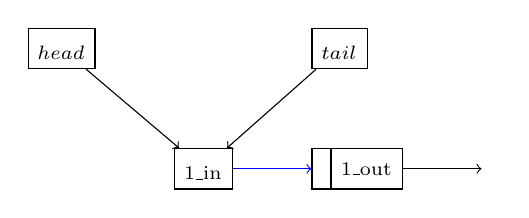
\begin{tikzpicture}[
    pair/.style = {
      on chain,
      rectangle split,
      rectangle split horizontal,
      rectangle split parts=2,
      draw,
      anchor=center,
      text height=1.5ex,
    },
    perspointer/.style = {
      on chain,
      rectangle,
      draw,
      anchor=center,
      text height=1.5ex,
    },
    pointer/.style = {
      rectangle,
      draw,
      anchor=center,
      text height=1.5ex,
    },
    start chain=going right,
  ]

  % Linked List
  \node (l'1) [join={by ->}, perspointer,on chain] {$\locin{1}$};
  \node (l1pair) [join={by ->, draw=blue}, pair,on chain] {$\None$ \nodepart{two} $\locout{1}$};
  \node (null) [join={by ->, draw=black}, rectangle,on chain] {$\None$};

  % Head and tail
  \node (head) [pointer, above left=of l'1] {$\loc_{head}$};
  \node (tail) [pointer, above right=of l'1] {$\loc_{tail}$};
  \draw[->] (head) -- (l'1);
  \draw[->] (tail) -- (l'1);

  \end{tikzpicture}
  \caption{Queue after initialisation}
  \label{MSQTL:impl:figure:init}
\end{figure}


\begin{figure}[h]
  \centering
  \begin{subfigure}{\textwidth}
    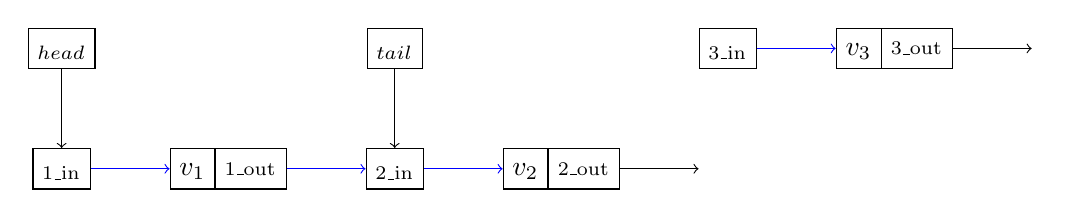
\begin{tikzpicture}[
      pair/.style = {
        on chain,
        rectangle split,
        rectangle split horizontal,
        rectangle split parts=2,
        draw,
        anchor=center,
        text height=1.5ex,
      },
      perspointer/.style = {
        on chain,
        rectangle,
        draw,
        anchor=center,
        text height=1.5ex,
      },
      pointer/.style = {
        rectangle,
        draw,
        anchor=center,
        text height=1.5ex,
      },
      start chain=going right,
    ]

    % Linked List
    \node (l'1) [join={by ->}, perspointer,on chain] {$\locin{1}$};
    \node (l1pair) [join={by ->, draw=blue}, pair,on chain] {$v_1$ \nodepart{two} $\locout{1}$};
    \node (l'2) [join={by ->, draw=blue}, perspointer,on chain] {$\locin{2}$};
    \node (l2pair) [join={by ->, draw=blue}, pair,on chain] {$v_2$ \nodepart{two} $\locout{2}$};
    \node (null) [join={by ->, draw=black}, rectangle,on chain] {$\None$};

    \node (l'3) [perspointer, above right=of l2pair] {$\locin{3}$};
    \node (l3pair) [join={by ->, draw=blue}, pair,on chain] {$v_3$ \nodepart{two} $\locout{3}$};
    \node (null) [join={by ->, draw=black}, rectangle,on chain] {$\None$};

    % Head and tail
    \node (head) [pointer, above=of l'1] {$\loc_{head}$};
    \node (tail) [pointer, above=of l'2] {$\loc_{tail}$};
    \draw[->] (head) -- (l'1);
    \draw[->] (tail) -- (l'2);

    \end{tikzpicture}
    \caption{Queue after creating the new node $(\locin{3}, v_3, \locout{3})$ to be added to the queue.}
    \label{MSQTL:impl:figure:enqueue:a}
    \vspace{2em}
  \end{subfigure}
  \begin{subfigure}{\textwidth}
    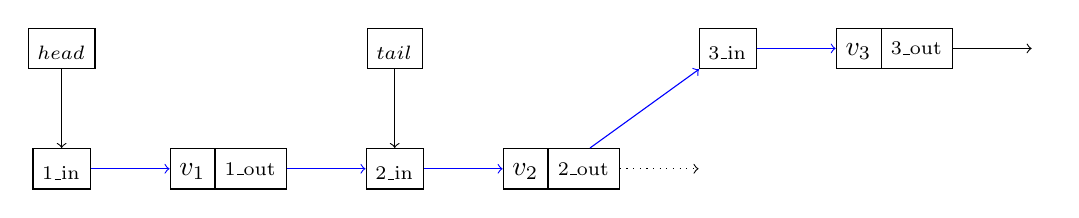
\begin{tikzpicture}[
      pair/.style = {
        on chain,
        rectangle split,
        rectangle split horizontal,
        rectangle split parts=2,
        draw,
        anchor=center,
        text height=1.5ex,
      },
      perspointer/.style = {
        on chain,
        rectangle,
        draw,
        anchor=center,
        text height=1.5ex,
      },
      pointer/.style = {
        rectangle,
        draw,
        anchor=center,
        text height=1.5ex,
      },
      start chain=going right,
    ]

    % Linked List
    \node (l'1) [join={by ->}, perspointer,on chain] {$\locin{1}$};
    \node (l1pair) [join={by ->, draw=blue}, pair,on chain] {$v_1$ \nodepart{two} $\locout{1}$};
    \node (l'2) [join={by ->, draw=blue}, perspointer,on chain] {$\locin{2}$};
    \node (l2pair) [join={by ->, draw=blue}, pair,on chain] {$v_2$ \nodepart{two} $\locout{2}$};
    \node (null) [join={by ->, dotted, draw=black}, rectangle,on chain] {\textcolor{gray}{$\None$}};

    \node (l'3) [perspointer, above right=of l2pair] {$\locin{3}$};
    \node (l3pair) [join={by ->, draw=blue}, pair,on chain] {$v_3$ \nodepart{two} $\locout{3}$};
    \node (null) [join={by ->, draw=black}, rectangle,on chain] {$\None$};
    \draw[->, draw=blue] (l2pair) -- (l'3);

    % Head and tail
    \node (head) [pointer, above=of l'1] {$\loc_{head}$};
    \node (tail) [pointer, above=of l'2] {$\loc_{tail}$};
    \draw[->] (head) -- (l'1);
    \draw[->] (tail) -- (l'2);

    \end{tikzpicture}
    \caption{Queue after adding the new node to linked list.}
    \label{MSQTL:impl:figure:enqueue:b}
    \vspace{2em}
  \end{subfigure}
  \begin{subfigure}{\textwidth}
    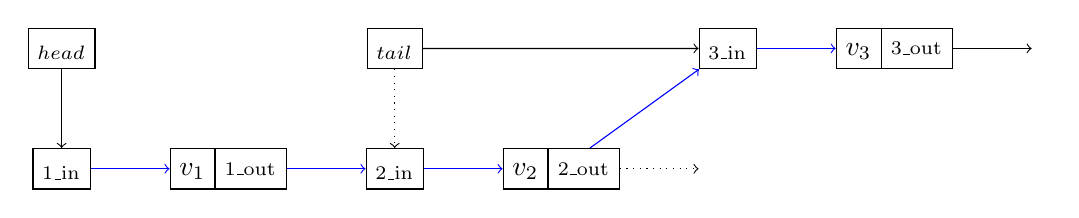
\begin{tikzpicture}[
      pair/.style = {
        on chain,
        rectangle split,
        rectangle split horizontal,
        rectangle split parts=2,
        draw,
        anchor=center,
        text height=1.5ex,
      },
      perspointer/.style = {
        on chain,
        rectangle,
        draw,
        anchor=center,
        text height=1.5ex,
      },
      pointer/.style = {
        rectangle,
        draw,
        anchor=center,
        text height=1.5ex,
      },
      start chain=going right,
    ]

    % Linked List
    \node (l'1) [join={by ->}, perspointer,on chain] {$\locin{1}$};
    \node (l1pair) [join={by ->, draw=blue}, pair,on chain] {$v_1$ \nodepart{two} $\locout{1}$};
    \node (l'2) [join={by ->, draw=blue}, perspointer,on chain] {$\locin{2}$};
    \node (l2pair) [join={by ->, draw=blue}, pair,on chain] {$v_2$ \nodepart{two} $\locout{2}$};
    \node (null) [join={by ->, dotted, draw=black}, rectangle,on chain] {\textcolor{gray}{$\None$}};

    \node (l'3) [perspointer, above right=of l2pair] {$\locin{3}$};
    \node (l3pair) [join={by ->, draw=blue}, pair,on chain] {$v_3$ \nodepart{two} $\locout{3}$};
    \node (null) [join={by ->, draw=black}, rectangle,on chain] {$\None$};
    \draw[->, draw=blue] (l2pair) -- (l'3);

    % Head and tail
    \node (head) [pointer, above=of l'1] {$\loc_{head}$};
    \node (tail) [pointer, above=of l'2] {$\loc_{tail}$};
    \draw[->] (head) -- (l'1);
    \draw[->, dotted] (tail) -- (l'2);
    \draw[->] (tail) -- (l'3);

    \end{tikzpicture}
    \caption{Queue after swinging tail pointer to the new node.}
    \label{MSQTL:impl:figure:enqueue:c}
  \end{subfigure}
  \caption{Enqueuing an element to a queue with one element.}
  \label{MSQTL:impl:figure:enqueue}
\end{figure}


\begin{figure}[h]
  \centering
  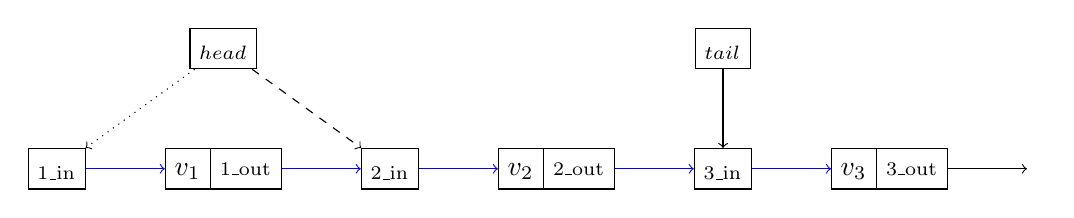
\begin{tikzpicture}[
    pair/.style = {
      on chain,
      rectangle split,
      rectangle split horizontal,
      rectangle split parts=2,
      draw,
      anchor=center,
      text height=1.5ex,
    },
    perspointer/.style = {
      on chain,
      rectangle,
      draw,
      anchor=center,
      text height=1.5ex,
    },
    pointer/.style = {
      rectangle,
      draw,
      anchor=center,
      text height=1.5ex,
    },
    start chain=going right,
  ]

  % Linked List
  \node (l1in) [join={by ->}, perspointer,on chain] {$\locin{1}$};
  \node (l1pair) [join={by ->, draw=blue}, pair,on chain] {$v_1$ \nodepart{two} $\locout{1}$};
  \node (l2in) [join={by ->, draw=blue}, perspointer,on chain] {$\locin{2}$};
  \node (l2pair) [join={by ->, draw=blue}, pair,on chain] {$v_2$ \nodepart{two} $\locout{2}$};
  \node (l3in) [join={by ->, draw=blue}, perspointer,on chain] {$\locin{3}$};
  \node (l3pair) [join={by ->, draw=blue}, pair,on chain] {$v_3$ \nodepart{two} $\locout{3}$};
  \node (null) [join={by ->, draw=black}, rectangle,on chain] {$\None$};

  % Head and tail
  \node (head) [pointer, above=of l1pair] {$\loc_{head}$};
  \node (tail) [pointer, above=of l3in] {$\loc_{tail}$};
  \draw[->, dotted] (head) -- (l1in);
  \draw[->, dashed] (head) -- (l2in);
  \draw[->] (tail) -- (l3in);

  \end{tikzpicture}
  \caption{Dequeueing an element ($v_2$) from a queue with two elements ($v_2$, $v_3$). The dotted line represents the state before the dequeue, and the dashed line is the state after dequeuing.}
  \label{MSQTL:impl:figure:dequeue}
\end{figure}

\begin{minted}[linenos=true, escapeinside=||,mathescape=true]{ocaml}
|$\label{}$|  |$ \initialise \eqdef $|
|$\label{}$|    |$ \Let node = \Ref(\None, \Ref(\None)) in $|
|$\label{}$|    |$ \Let H\_lock = newlock \TT in $|
|$\label{}$|    |$ \Let T\_lock = newlock \TT in $|
|$\label{}$|    |$ \Ref((\Ref(node), \Ref(node)), (H\_lock, T\_lock)) $|
\end{minted}

\begin{minted}[linenos=true, escapeinside=||,mathescape=true]{ocaml}
|$\label{}$|  |$ \enqueue \ Q \ value \eqdef $|
|$\label{}$|    |$ \Let node = \Ref(\Some value, \Ref(\None)) in $|
|$\label{}$|    |$ \acquire (\Snd (\Snd (\deref Q))); $|
|$\label{}$|    |$ \Snd (\deref(\deref(\Snd (\Fst(\deref Q))))) \gets node; $|
|$\label{}$|    |$ \Snd (\Fst (\deref Q)) \gets node; $|
|$\label{}$|    |$ \release (\Snd (\Snd (\deref Q))) $|
\end{minted}

\begin{minted}[linenos=true, escapeinside=||,mathescape=true]{ocaml}
|$\label{}$|  |$ \dequeue \ Q \eqdef $|
|$\label{}$|    |$ \acquire (\Fst (\Snd (\deref Q))); $|
|$\label{}$|    |$ \Let node = \deref (\Fst (\Fst (\deref Q))) in $|
|$\label{}$|    |$ \Let new\_head = \deref (\Snd(\deref node)) in $|
|$\label{}$|    |$ \If new\_head = \None then $|
|$\label{}$|      |$ \release (\Fst (\Snd(\deref Q))); $|
|$\label{}$|      |$ \None $|
|$\label{}$|    |$ \Else $|
|$\label{}$|      |$ \Let value = \Fst (\deref new\_head) in $|
|$\label{}$|      |$ \Fst (\Fst (\deref Q)) \gets new\_head; $|
|$\label{}$|      |$ \release (\Fst (\Snd (\deref Q))); $|
|$\label{}$|      |$ value $|
\end{minted}

% \begin{align*}
%   \langkw{let} \initialise := &\\
%                     & \Let node = \Ref(\None, \Ref(\None)) in\\
%                     & \Let H\_lock = newlock \TT in\\
%                     & \Let T\_lock = newlock \TT in\\
%                     & \Ref((\Ref(node), \Ref(node)), (H\_lock, T\_lock))
% \end{align*}

% \begin{align*}
%   \langkw{let} \enqueue \ Q \ value :=&\\
% 		& \Let node = \Ref(\Some value, \Ref(\None)) in\\
% 		& \acquire (\Snd (\Snd (\deref Q)));\\
% 		& \Snd (\deref(\deref(\Snd (\Fst(\deref Q))))) \gets node;\\
% 		& \Snd (\Fst (\deref Q)) \gets node;\\
% 		& \release (\Snd (\Snd (\deref Q)))
% \end{align*}

% \begin{align*}
%   \langkw{let} \dequeue \ Q :=&\\
% 		& \acquire (\Fst (\Snd (\deref Q)));\\
% 		& \Let node = \deref (\Fst (\Fst (\deref Q))) in\\
% 		& \Let new\_head = \deref (\Snd(\deref node)) in\\
% 		& \If new\_head = \None then\\
% 			& \hspace{20pt} \release (\Fst (\Snd(\deref Q)));\\
% 			& \hspace{20pt} \None\\
% 		& \Else\\
% 			& \hspace{20pt} \Let value = \Fst (\deref new\_head) in\\
% 			& \hspace{20pt} \Fst (\Fst (\deref Q)) \gets new\_head;\\
% 			& \hspace{20pt} \release (\Fst (\Snd (\deref Q)));\\
%       & \hspace{20pt} value
% \end{align*}


\section{Sequential Specification}\label{MSQTL:Sequential}

Let us first prove a specification for the two-lock michael scott queue in the simple case where we don't allows for concurrency. In this case, we know that only a single thread will interact with the queue at any given point in a sequential manner. This means that we give a specification that tracks the exact contents of the queue. To this end, we shall define the abstract state of the queue, denoted $xs_v$ as a list of \heaplang values. I.e. $xs_v : \List \ \Val$. We adopt the convention that enqueueing an element is done by adding it to the front of the list, and dequeueing removes the last element of the list (if such an element exists). The reason for this choice is purely technical.

Since the queue uses two locks, we will get two ghost names; one for each lock. For this specification, these are the only two ghost names we will need. However, for the later specifications, we will use more resource algebra, and will need more ghost names. Thus, to ease notation, we shall define the type "$SeqQgnames$" whose purpose is to keep track of the ghost names used for a specific queue. Since we only have two ghost names for this specification, element of $SeqQgnames$ will simply be pairs. For an element $Q_\gname \in SeqQgnames$, the first element of the pair, written $Q_\gname.\gname_{Hlock}$, will contain the ghost name for the head lock, and the second element, $Q_\gname.\gname_{Tlock}$, the ghost name for the head lock.

The sequential specification we wish to prove is the following:
\begin{align*}
  &\Exists \isqueueseq : \Val \to \List \ \Val \to SeqQgnames \to \Prop.\\
  &\quad\quad\hoare{\TRUE}{\initialise \TT}{v_q . \Exists Q_\gname. \isqueueseq\ v_q\ []\ Q_\gname}\\
  &\land\quad\All v_q, v, xs_v, Q_\gname. \hoare{\isqueueseq \; v_q \; xs_v \; Q_\gname}{\enqueue\ v_q\ v}{w . \isqueueseq\ v_q\ (v :: xs_v)\ Q_\gname}\\
  &\land\quad\All v_q, xs_v, Q_\gname. \hoareV[t]{\isqueueseq \; v_q \; xs_v \; Q_\gname}{\dequeue\ v_q}{v . \begin{array}{l}(xs_v = [] \ast v = \None \ast \isqueueseq\ v_q\ xs_v\ Q_\gname) \; \lor\\ (\Exists x_v, xs_v' . xs_v = xs_v' \catenate [x_v] \ast v = \Some x_v \ast \isqueueseq\ v_q\ xs_v'\ Q_\gname) \end{array}}
\end{align*}

The predicate $\isqueueseq \; v_q \; xs_v \; Q_\gname$ captures that the value $v_q$ is a queue, whose content matches that of our abstract representation $xs_v$, and the queue uses the ghost names described by $Q_\gname$. Note that the $\isqueueseq$ predicate is not required to be persistent, hence it cannot be duplicated and given to multiple threads. This is the sense in which this specification is sequential.

\section{Proving the Sequential Specification}
\subsection[The isqueueseq predicate]{The $\isqueueseq$ Predicate}
To prove the specification we must give a specific $\isqueueseq$ predicate. To help guide us in designing this, we give the following observations about the behaviour of the implementation.
\begin{enumerate}
  \item\label{MSQTL:insights:head} Head always points to the first node in the queue.
  \item\label{MSQTL:insights:tail} Tail always points to either the last or second last node in the queue.
  \item\label{MSQTL:insights:persistent} All but the last pointer in the queue (the pointer to $\None$) never change.
\end{enumerate}

Observation \ref{MSQTL:insights:tail} captures the fact that, while enqueueing, a new node is first added to the linked list, and then later the tail is updated to point to the newly added node. Since only one thread can enqueue a node at a time (due to the lock), then the tail will only ever point to the last or second last due to the above. However, in a sequential setting, the tail will always appear to point to the last node, as no one can inspect the queue while the tail points to the second last.

Insight \ref{MSQTL:insights:persistent} means that we can mark all pointers in the queue (except the pointer to the null node) as persistent. This is technically not needed in the sequential case, but we will incorporate it now, as we will need it in the concurrent setting.

\begin{align*}
  \isqueueseq \; v_q \; xs_v \; Q_\gname \eqdef &\Exists \loc_{queue}, \loc_{head}, \loc_{tail} \in \Loc . \Exists h_{lock}, t_{lock} \in \Val . \\
  &v_q = \loc_{queue} \ast \loc_{queue} \mapsto^{\persistently} ((\loc_{head}, \loc_{tail}), (h_{lock}, t_{lock})) \ast\\
  &\Exists xs_{queue} \in \List (\Loc \times \Val \times \Loc) . \Exists x_{head}, x_{tail} \in (\Loc \times \Val \times \Loc) .\\
	&proj\_val \ xs_{queue} = wrap\_some \ xs_v \ast\\
	&\isLL (xs_{queue} \catenate [x_{head}]) \ast\\
	&\loc_{head} \mapsto (\nIn{x_{head}}) \ast\\
	&\loc_{tail} \mapsto (\nIn{x_{tail}}) \ast isLast \ x_{tail} \ (xs_{queue} \catenate [x_{head}]) \ast\\
	&isLock \ Q_\gname.\gname_{Hlock} \ h_{lock} \ \TRUE \ast\\
	&isLock \ Q_\gname.\gname_{Tlock} \ t_{lock} \ \TRUE.
\end{align*}

This $\isqueueseq$ predicate states that the value $v_q$ is a location, which persistently points to the structure containing the head, the tail, and the two locks. It also connects the abstract state $xs_v$ with the concrete state by stating that if you strip away the locations in $xs_{queue}$ (achieved by $proj\_val$) and wrap the values in the abstract state $xs_v$ in $\Some$ (achieved by $wrap\_some$), then the lists become equal.\\
Next, the predicate specifies the concrete state. There is some head node $x_{head}$, which the head points to. This head node and the nodes in $xs_{queue}$ form the underlying linked list (specified using the $\isLL$ predicate below). There is also a tail node, which is the last node in the linked list, and the tail points to this node. The proposition $isLast\ x\ xs$ simply asserts the existence of some $xs'$, so that $xs = x :: xs'$.\\
Finally, we have the isLock predicate for our two locks. Since we are in a sequential setting, then the locks are superfluous, hence they simply protect $\TRUE$.

The $\isLL$ predicate essentially creates the structure seen in the examples of section \ref{section:two_lock:impl}. It is defined in two steps. Firstly, we create all the persistent pointers in the linked list using the $\isLLchain$ predicate. Note that this in effect makes $\isLLchain \ xs$ persistent for all $xs$.
\begin{definition}[Linked List Chain Predicate]
  \begin{align*}
    \isLLchain{[]} \equiv& \TRUE\\
    \isLLchain{[x]} \equiv& \nIn{x} \mapsto^{\persistently} (\nVal{x}, \nOut{x})\\
    \isLLchain{x :: x' :: xs} \equiv& \nIn{x} \mapsto^{\persistently} (\nVal{x}, \nOut{x}) \ast \nOut{x'} \mapsto^{\persistently} \nIn{x} \ast \isLLchain{x' :: xs}
  \end{align*}
\end{definition}

Then, to define $\isLL$, we add that the last node in the linked list points to $\None$.
\begin{definition}[Linked List Predicate]
  \begin{align*}
    \isLL{[]} \equiv& \TRUE\\
    \isLL{x :: xs} \equiv& \nOut{x} \mapsto \None \ast \isLLchain{x :: xs}
  \end{align*}
\end{definition}

For instance, if we wanted to capture the linked list in figure \ref{MSQTL:impl:figure:enqueue:c}, we would use the list $xs = [(\locin{3}, v_3, \locout{3}); (\locin{2}, v_2, \locout{2});  (\locin{1}, v_1, \locout{1})]$. $\isLL{xs}$ will expand to $\locout{3} \mapsto \None \ast \isLLchain{xs}$, and $\isLLchain{xs}$ expands to
\begin{align*}
  &\locin{3} \mapsto^{\persistently} (x_3, \locout{3}) \ast \locout{2}	\mapsto^{\persistently} \locin{3}\ast\\
  &\locin{2} \mapsto^{\persistently} (x_2, \locout{2}) \ast \locout{1}\mapsto^{\persistently} \locin{2} \ast\\
  &\locin{1} \mapsto^{\persistently} (x_1, \locout{1})
\end{align*}
Note how this matches the structure of the linked list in figure \ref{MSQTL:impl:figure:enqueue:c}.

\subsection{Proof outline}

\subsubsection{Initialise}
Proving the initialise spec amounts to stepping through the code, giving us the required resources, and then using these to create an instance of $\isqueueseq$ with the obtained resources. To begin with, we step through the lines creating the first node $x_1$, giving us locations $\locin{1}$, $\locout{1}$ with $\locout{1} \mapsto \None$ and $\locin{1} \mapsto (\None, \locout{1})$. We can then update the latter points-to predicate to become persistent, giving us $\locin{1} \mapsto^{\persistently} (\None, \locout{1})$. We then step to the creation of the two locks, where we shall use the newlock specification asserting that the locks should protect $\TRUE$. This gives us two ghost names, $\gname_{Tlock}$, $\gname_{Tlock}$, which we will collect in a $SeqQgnames$ pair, $Q_\gname$.
Next, we step through the allocations of the head, tail, and queue, which gives us locations $\loc_{head}$, $\loc_{tail}$, $\loc_{queue}$, such that both $\loc_{head}$ and $\loc_{tail}$ point to node $x_1$, and such that $\loc_{queue}$ points to the structure containing the head, tail, and two locks. This last points to predicate we update to become persistent.
With this, we now have all the resources needed to prove the post-condition: $\Exists Q_\gname . \isqueueseq \ \loc_{queue} \ Q_\gname$. Proving this follows by a sequence of framing away the resources we obtained and instantiating existentials with the values we got above. Most noteworthy, we pick the empty list for $xs_{queue}$, and node $x_1$ for $x_{head}$ and $x_{tail}$.


\subsubsection{Enqueue}
\todo{add line numbers to code, and refer to them in proof}
For enqueue, we get in our pre-condition $\isqueueseq \; v_q \; xs_v \; Q_\gname$, and we wish to that, if we run $\enqueue\ v_q\ v$, then we will get $\isqueueseq\ v_q\ (v :: xs_v)\ Q_\gname$. The proposition $\isqueueseq \; v_q \; xs_v \; Q_\gname$ gives us all the resources we will need to step through the code.
Firstly, we create a new node, node $x_{new}$, with $\nVal{x_{new}} = v$.
We then have to acquire the lock, which will just give us $\TRUE$.

The next line adds node $x_new$ to the linked list, by first finding the tail, from the queue pointer $\loc_{queue}$, and then finding the node that the tail points to, denoted $x_{tail}$, and finally writing updating the out location of $x_{tail}$ to point to $x_new$. The resources needed to do this are all described in $\isqueueseq \; v_q \; xs_v \; Q_\gname$. Firstly, it tells us that $\loc_{queue}$ points to the structure containing $\loc_{tail}$. Secondly, it tells us that $\loc_{tail}$ points to $x_{tail}$, which is the last node in the linked list ($xs_{queue} \catenate [x_{head}]$). Thirdly, since we know that $x_{tail}$ is the last node in the linked list, then by the $\isLL$ predicate, we know that $x_{tail}$ points to $\None$ and that it has the node-like structure described by $\isLLchain$. This is all we need to step through the line, adding $x_{new}$ to the linked list. After performing the write, we then get that $x_{tail}$ points to $x_{new}$, instead of $\None$. We make this points-to predicate persistent.

The next line swings the tail to $x_{new}$. As describe above, we already know that $\loc_{tail}$ points to $x_{tail}$, so we have the required resources to perform the write. Afterwards, we get that $\loc_{tail}$ points to $x_{new}$.

Finally, we release the lock using the release specification (and we simply give back $\TRUE$), and the only thing left is to prove the postcondition: $\isqueueseq\ v_q\ (v :: xs_v)\ Q_\gname$. For the existentials, we shall pick the ones we got from the precondition, with the exception for $xs_{queue}$ and $x_{tail}$. For $xs_{queue}$, we shall use the same $xs_{queue}$ we got from the precondition, but with $xs_new$ cons'ed to it, and for $x_{tail}$, we chose the new tail node: $x_{new}$. With these choices, proving $\isqueueseq\ v_q\ (v :: xs_v)\ Q_\gname$ is fairly straightforward.

\subsubsection{Dequeue}

For $\dequeue\ v_q$, our precondition is $\isqueueseq \; v_q \; xs_v \; Q_\gname$, and our post condition states that either the queue is empty, or there is a tail element which is returned by the function, and removed from the queue.

Stepping through the function, we first do the superfluous acquire. Next, we get the head node $x_{head}$ through the queue pointer $\loc_{queue}$. As described above for Enqueue, we get the resource to do this through $\isqueueseq \; v_q \; xs_v \; Q_\gname$. The $\isqueueseq$ predicate also tells us that $x_{head}$ is a node in the linked list (described by the $\isLL$ predicate), hence we can step through the code in the next line, which finds the node that $x_{head}$ is pointing to. Now, depending on whether or not the queue is empty, $x_{head}$ either points to $\None$, or some node $x_{head\_next}$. Thus, we shall perform a case analysis on $xs_{queue}$.

\textbf{$xs_{queue}$ is empty}: In this case, we will have that $\isLL [x_{head}]$, which tells us that $x_head$ points to $\None$. Hence, the "then" branch of the "if" will be taken. This branch simply releases the lock and returns $\None$. In this case, we prove the first disjunction in the post-condition. Since $xs_v$ is reflected in $xs_{queue}$, then we will be able to conclude that $xs_v$ is empty, and since we haven't modified the queue, we can create $\isqueueseq \; v_q \; xs_v \; Q_\gname$ using the same resources we got from the pre-condition.

\textbf{$xs_{queue}$ is not empty}: In this case, we can conclude that there must be some node $x_{head\_next}$, which is the first node in $xs_{queue}$. I.e. $xs_{queue} = xs'_{queue} \catenate [x_{head\_next}]$. We can thus use the $\isLL$ predicate to conclude that $x_{head}$ must point to $x_{head\_next}$. Hence the else branch will be taken. Since $x_{head\_next}$ is part of the linked list, then $\isLL$ tells us it has the node-like structure, allowing us to extract its value in the first line of the else branch.\\
In the next line, we make the head pointer, $\loc_{head}$ point to $x_{head\_next}$, and we have the resource to do this through $\isqueueseq \; v_q \; xs_v \; Q_\gname$.\\
Finally, we release the lock and return the value we got from $x_{head\_next}$. We must now prove the post-condition, and this time we prove the second disjunct. Since $xs_v$ is reflected in $xs_{queue}$, then it must also be the case that $xs_v$ is non-empty, and it has a first element, $x_v$, which is related to the first element of $xs_{queue}$, i.e. $x_{head\_next}$. This allows us to conclude that the returned value ($\nVal{x_{head\_next}}$) is exactly $x_v$, but wrapped in a $\Some$, as we had to prove.
Finally, we must prove $\isqueueseq\ v_q\ xs_v'\ Q_\gname$, where $xs_v'$ is $xs_v$ but with $x_v$ removed. For the existentials, we pick the same values we got from the precondition, wit the exception of $xs_{queue}$ and $x_{head}$. For $xs_{queue}$ we pick the same $xs_{queue}$ we got from the precondition, but with the first element, $x_{head\_next}$ removed. By doing this, $xs_{queue}$ will be reflexed in $xs_v'$. For $x_head$, we pick the new head, which we have obtained that $\loc_{head}$ points to: $x_{head\_next}$. With these choices, we can prove the predicate.



\section{Concurrent Specification}\label{MSQTL:Concurrent}
For the concurrent specification, we will need the predicate capturing the queue (here denoted $\isqueueconc$) to be duplicable. To achieve this, we shall initially give up on tracking the abstract state of the queue, and instead add a predicate $\Phi$, which we will ensure holds for all elements of the queue. In this way, when dequeueing, we at least know that if we get some value, then $\Phi$ holds of this value. The specification we wish to prove is as follows.
\begin{align*}
  &\Exists \isqueueconc : (\Val \to \Prop) \to \Val \to ConcQgnames \to \Prop.\\
  &\All \Phi : \Val \to \Prop.\\
  &\quad\quad \All v_q, Q_\gname . \isqueueconc \ \Phi \ v_q \ Q_\gname \implies \persistently \isqueueconc \ \Phi \ v_q \ Q_\gname\\
  &\land\quad\hoare{\TRUE}{\initialise \TT}{v_q . \Exists Q_\gname. \isqueueconc\ \Phi \ v_q \ Q_\gname}\\
  &\land\quad\All v_q, v, Q_\gname. \hoare{\isqueueconc \ \Phi \ v_q \ Q_\gname \ast \Phi \ v}{\enqueue\ v_q\ v}{v . \TRUE}\\
  &\land\quad\All v_q, Q_\gname. \hoare{\isqueueconc \ \Phi \ v_q \ Q_\gname}{\dequeue\ v_q}{v . v = \None \lor (\Exists x_v. v = \Some x_v \ast \Phi \ x_v)}
\end{align*}
Note that the type of the collection of ghost names here is $ConcQgnames$, as we will require more ghost names than before. The new ghost names are used for "tokens" which are introduced in the following section.

\section{Proving the Concurrent Specification}
\subsection[The isqueueconc predicate]{The $\isqueueconc$ Predicate}
As we did for the sequential specification, we note here some useful observations about the implementation.
\begin{enumerate}
  \item\label{MSQTL:insights:oldnodes} Nodes in the linked list are never deleted. Hence, the linked list only ever grows.
  \item\label{MSQTL:insights:lag} The tail can lag one node behind Head.
  \item\label{MSQTL:insights:states} At any given time, the queue is in one of four states:
    \begin{enumerate}
      \item\label{MSQTL:insights:state:static} No threads are interacting with the queue (\StaticState)
      \item\label{MSQTL:insights:state:enqueue} A thread is enqueueing (\EnqueueState)
      \item\label{MSQTL:insights:state:dequeue} A thread is dequeuing (\DequeueState)
      \item\label{MSQTL:insights:state:both} A thread is enqueueing and a thread is dequeuing (\BothState)
    \end{enumerate}
\end{enumerate}

Observation \ref{MSQTL:insights:lag} might seem a little surprising, and indeed it stands in contrast to property 5 in \cite{DBLP:conf/podc/MichaelS96}, which states that the tail never lags behind head. I also didn't realise this possibility until a proof attempt using a model that "forgot" old nodes lead to an unprovable case (see section \ref{MSQTL:Discussion:xs_old}). The situation can occur when the queue is empty, and a thread performs an incomplete enqueue; it attaches the new node to the end, but before it can swing the tail to this new node, another thread performs a dequeue, which dequeues this new node, swinging the head to it. Now the tail is lagging a node behind the head.

It is not possible for the tail to point more than one node behind the head, as in order for this to happen, more nodes must be enqueued, but this can't happen before the current enqueue finishes, which will update the tail and bring it up to speed with the head.

Fortunately, this isn't an issue for safety, but a consequence of this possibility is that when modelling the queue, we must remember at least one "old" node (i.e. a dequeued node), as the tail might be pointing to this node. For the sake of simplicity in the model, the choice is made to remember an arbitrary amount of old nodes, which is represented by the list $xs_{old}$.

Observation \ref{MSQTL:insights:states} is a simple consequence of the implementation using two locks.

Since we want $\isqueueconc$ to be persistent, then we cannot directly state the points-to predicates as we did in the sequential case. However, we will still need all the same resources to be able to prove the specification. The solution is to have an invariant which describes the concrete state of the queue. In the proofs, when we need access to some resource, we shall then access it by opening the invariant. We now present the invariant and explain it afterwards.
\begin{definition}[Two-Lock M\&S-Queue Invariant]\label{MSQTL:spec:invariant}
  \begin{align*}
    &queue\_invariant \ \Phi \ \loc_{head} \ \loc_{tail} \ Q_\gname \eqdef\\
    &\Exists xs_v. All \ xs_v \ \Phi \ast &&\text{(abstract state)}\\
    &\Exists xs, xs_{queue}, xs_{old}, x_{head}, x_{tail} . &&\text{(concrete state)}\\
    &xs = xs_{queue} \catenate [x_{head}] \catenate xs_{old} \ast\\
    &\isLL \ xs \ast\\
    &proj\_val \ xs_{queue} = wrap\_some \ xs_v \ast\\
    &(\\
    &\quad\quad\loc_{head} \mapsto (\nIn{x_{head}}) \ast \loc_{tail} \mapsto (\nIn{x_{tail}}) \ast isLast \ x_{tail} \ xs \ast &&\text{(\StaticState)}\\
    &\quad\quad \ToknEQg \ast \ToknDQg \ast \TokUpdatedQg\\
    &\quad\lor\\
    &\quad\quad\loc_{head} \mapsto (\nIn{x_{head}}) \ast \loc_{tail} \mapsto^{\frac{1}{2}} (\nIn{x_{tail}}) \ast &&\text{(\EnqueueState)}\\
    &\quad\quad (isLast \ x_{tail} \ xs \ast \TokBeforeQg \lor isSndLast \ x_{tail} \ xs \ast \TokAfterQg) \ast\\
    &\quad\quad \TokEQg \ast \ToknDQg\\
    &\quad\lor\\
    &\quad\quad\loc_{head} \mapsto^{\frac{1}{2}} (\nIn{x_{head}}) \ast \loc_{tail} \mapsto (\nIn{x_{tail}}) \ast isLast \ x_{tail} \ xs \ast &&\text{(\DequeueState)}\\
    &\quad\quad \ToknEQg \ast \TokDQg \ast \TokUpdatedQg\\
    &\quad\lor\\
    &\quad\quad\loc_{head} \mapsto^{\frac{1}{2}} (\nIn{x_{head}}) \ast \loc_{tail} \mapsto^{\frac{1}{2}} (\nIn{x_{tail}}) \ast &&\text{(\BothState)}\\
    &\quad\quad (isLast \ x_{tail} \ xs \ast \TokBeforeQg \lor isSndLast x_{tail} xs \ast \TokAfterQg) \ast\\
    &\quad\quad \TokEQg \ast \TokDQg\\
    &)
  \end{align*}
\end{definition}
In contrast to the sequential specification, the abstract state is now existentially quantified, hence the exact contents of the queue are not tracked. Instead, we have added the proposition $All \ xs_v \ \Phi$, which states that all values in $xs_v$ (i.e. the values currently in the queue) satisfy the predicate $\Phi$. This will allow us to conclude that dequeued values satisfy $\Phi$.\\
The concrete state of the queue is still reflected in the abstract state through projecting out the values of the nodes ($proj\_val$), and wrapping the values in the queue in $\Some$ ($wrap\_some$). Another difference is that we now also keep track of an arbitrary number of "old" nodes; nodes that are behind the head node, $x_{head}$. As discussed above, this inclusion is due to observation \ref{MSQTL:insights:lag}.\\
As before, we also assert that the concrete state forms a linked list, as described by the $\isLL$ predicate.\\
The final part of the invariant describes the four possible states of the queue, as described in \ref{MSQTL:insights:states}. Since the resources used by the queue are inside an invariant, and enqueueing/dequeueing threads need to access the resources of the queue multiple times, then we will have to open and close the invariant multiple times. Each time we open the invariant, the existentially quantified variables will not be the same as those from early accesses of the invariant (as they are existentially quantified). Thus, the threads must be able to "match up" variables from previous accesses to later accesses. The way we shall achieve this is by allowing threads to keep a \textit{fraction} of the points-to predicate that it is using. For instance, an enqueuing thread will have to access the points-to predicate concerning $\loc_{tail}$ multiple times, and in between accesses of the invariant, it can get to keep half of the points-to predicate. Thus, when it opens the invariant later, it will have $\loc_{tail} \mapsto^{\frac{1}{2}} \nIn{x_{tail}}$ from an earlier access, and it will obtain the existence of some new $x_{tail}'$, such that $\loc_{tail} \mapsto^{\frac{1}{2}} \nIn{x_{tail}'}$. Combining the two points-to predicates allows us to conclude that $\nIn{x_{tail}} = \nIn{x_{tail}'}$. In this way, we can match up variables from earlier accesses to variables in later accesses.\\
In the \StaticState{} state where no thread is interacting with the queue, the queue owns all of the points-to predicates concerning the head and tail.\\
In the \EnqueueState{} state, the enqueueing thread owns half of the tail pointer, and we distinguish between two cases, as discussed in \ref{MSQTL:insights:tail}: either the enqueueing thread has yet to add the new node to the linked list and $x_{tail}$ is still the last node, or the new node has been added, but the tail pointer hasn't been updated, meaning that $x_{tail}$ is the second last node ($isSndLast$ is defined similarly to $isLast$).\\
In the \DequeueState{} state, the dequeueing thread owns half of the head pointer, and the tail is as in the \StaticState{} state.\\
Finally, the \BothState{} state is essentially a combination of the \EnqueueState{} and \DequeueState{} states.

To track which state the queue is in, we use \textit{tokens}. Tokens are defined using the exclusive resource algebra on the singleton set: $\exm{\TT}$. This resource algebra only has one valid element, and combining two elements will give the non-valid element $\bot$. Thus, if we own a particular token, then, upon opening the invariant, we can rule out certain states simply because they mention the token we own.\\
We will use several tokens, each of which is the valid element of their own instance of $\exm{\TT}$. Different instances are distinguish between using ghost names. Hence, each token will be represented by a ghost name. As we did for the sequential specification, we group these ghost names into a tuple $\Qg$, and write, for instance $\TokEQg$ to refer to the valid element of a particular instance. We proceed to explain the meaning of each of the tokens used in the invariant.
\begin{itemize}
  \item $\ToknEQg$ represents that no threads are enqueueing.
  \item $\TokEQg$ represents that a thread is enqueueing.
  \item $\ToknDQg$ represents that no threads are dequeueing.
  \item $\TokDQg$ represents that a thread is dequeueing.
  \item $\TokBeforeQg$ represents that an enqueueing thread has not yet added the new node to the linked list.
  \item $\TokAfterQg$ represents that an enqueueing thread has added the new node to the linked list, but not yet swung the tail.
  \item $\TokUpdatedQg$ is defined as $\TokBeforeQg \ast \TokAfterQg$, and represents that the queue is up to date.
\end{itemize}


\textbf{Note}: The concurrent specification for the two-lock Michael Scott Queue \textit{can} be proven using the queue invariant \ref{MSQTL:spec:invariant}, and the proof outline below will also be using this. However, a simpler (but arguably less intuitive) queue invariant was discovered. This simpler invariant is equivalent to \ref{MSQTL:spec:invariant} and has the benefit of being easier to work with in the mechanised proofs. Thus, in the mechanised proofs, the simpler variant is used. The simpler variant can be found in the appendix \todo{add appendix}.

With this, we can now give our definition of $\isqueueconc$. In the below, we let $\Nl$ be some namespace.
\begin{align*}
  \isqueueconc \; \Psi \; v_q \; \Qg \eqdef &\Exists \loc_{queue}, \loc_{head}, \loc_{tail} \in \Loc . \Exists h_{lock}, t_{lock} \in \Val . \\
  &v_q = \loc_{queue} \ast \loc_{queue} \mapsto^{\persistently} ((\loc_{head}, \loc_{tail}), (h_{lock}, t_{lock})) \ast\\
	&\knowInv{\Nl.queue}{queue\_invariant \Phi \loc_{head} \loc_{tail} \Qg} \ast\\
	&isLock \ Q_\gname.\gname_{Hlock} \ h_{lock} \ (\TokDQg) \ast\\
	&isLock \ Q_\gname.\gname_{Tlock} \ t_{lock} \ (\TokEQg).
\end{align*}

In contrast to the sequential specification, the locks now protect $\TokEQg$ and $\TokDQg$. The idea is that, when an enqueueing thread obtains $t_{lock}$, they will obtain the $\TokEQg$ token, which allows them to conclude that the queue state is either \StaticState{} or \DequeueState{}. Similarly for a dequeueing thread. We now proceed to prove the specification using the above $\isqueueconc$ predicate.


\subsection{Proof outline}
Firstly, we must show that $\isqueueconc$ is persistent. This however follows from the fact that invariants are persistent, the $isLock$ predicates are persistent, persistent points-to predicates are persistent, and persistency is preserved by $\ast$ and quantifications (rules: persistently-sep, persistently-$\land$, persistently-$\exists$).

The proofs structure for the specifications are largely similar to the sequential counterparts. The major difference is that we don't have access to the resources all the time; we must get them from the invariant. Further we also have to keep track of which state we are in. For the proof outlines below, these points will be the main focus.

\subsubsection{Initialise}
We first step through the first line which gives us the sentinel node of the linked list. Next, we must create the two locks. To create the two tokens that the locks must protect, we use the ghost-alloc rule twice, which gives us two ghost names, one for each of the tokens. We put the ghost names into a tuple $\Qg$, and write $\TokEQg$ and $\TokDQg$ for the two ghost resources created by the ghost-alloc rule. We then create the locks, giving up the two tokens. Following this, we create the $\loc_{queue}$, $\loc_{head}$, and $\loc{tail}$ pointers. All that remains then is to prove the postcondition; the $\isqueueconc$ predicate. The persistent points-to predicate we got when we stepped through the code, and the $\isLock$ predicates we got when we created the locks. So all that remains is the invariant. We create the $queue\_invariant$ in the \StaticState{} state, most of which is analogous to the sequential specification. However, we will also need to supply the tokens required by the \StaticState{} state. Thus, we allocate the four tokens $\ToknEQg$, $\ToknDQg$, $\TokBeforeQg$, and $\TokAfterQg$ in the same way we allocated $\TokEQg$ and $\TokDQg$. We combine $\TokBeforeQg$ and $\TokAfterQg$ to get $\TokUpdatedQg$, and we now have all the tokens we need to create the $queue\_invariant$ in the \StaticState{} state. To create the invariant from $queue\_invariant$, we use the Inv-alloc rule (FUP).

\subsubsection{Enqueue}
We first step through the first line which gives us the new node $x_{new}$. We then acquire the tail lock $t_{lock}$, giving us $\TokEQg$. In the next line we must dereference the tail pointer, in order to get the tail node $x_tail$. This information, however, is inside the invariant. Invariant can only be opened if the expression being considered is atomic, but we can always make it atomic using the bind rule. Thus, we open the invariant, and since we have $\TokEQg$, we know that the queue is in state \StaticState{} or \DequeueState{}. In any case, we get that $\loc_{tail} \mapsto \nIn{x_{tail}}$, and that $x_{tail}$ is the last node in the linked list. We can then dereference $\loc_{tail}$, and must then close the invariant. We split up the points-to predicate $\loc_{tail} \mapsto \nIn{x_{tail}}$ in two, which leaves us with two of $\loc_{tail} \mapsto^{\frac{1}{2}} \nIn{x_{tail}}$. We keep one of them, and use the other to close the invariant in the before case of state \EnqueueState{} or \BothState{}, depending on which state we opened the invariant into. By doing this, we give up $\TokEQg$, but we gain $\ToknEQg$ and $\TokAfterQg$. We can now step to the point where $x_{tail}$'s out is updated to point to $x_{new}$. However, the points-to predicate concerning $\nOut{x_{tail}}$ isn't persistent, and is hence inside the invariant. We thus have to open the invariant again. Since we have $\ToknEQg$ and $\TokAfterQg$, we know that we are in the before case of either state \EnqueueState{} or \BothState{}. We now get a different tail node, $x_{tail}'$, with $\loc_{tail} \mapsto^{\frac{1}{2}} \nIn{x_{tail}'}$. However, since we kept $\loc_{tail} \mapsto^{\frac{1}{2}} \nIn{x_{tail}}$, we can combine these, allowing us to conclude that $\nIn{x_{tail}} = \nIn{x_{tail}'}$. Due to the structure of nodes (as described by $\isLL$), we can further conclude that $x_{tail} = x_{tail}'$. This now gives us that $\nOut{x_{tail}} \mapsto \None$, and we can perform the store, adding $x_{new}$ to the linked list. We now wish to close the invariant in the after case of either state \EnqueueState{} or \BothState{}, giving up $\TokAfterQg$, and obtaining $\TokBeforeQg$. When closing the invariant we shall pick as the abstract state $v :: xs_v$, where $v$ is the enqueued value, and $xs_v$ the abstract state we got when we opened the invariant. Note that in the pre-condition of the hoare-triple, we have $\Phi v$, hence we will be able to conclude $All (v :: xs_v) \Phi$. For the concrete state, we pick $x_{new} :: xs$, where $xs$ is the concrete state we got when we opened the invariant. With these choices, we can close the invariant.\\
The next line swings the tail pointer to $x_{new}$. But to perform this store, we must first know that $\loc_{tail}$ points to something. This resource is inside the invariant, so we must open the invariant one last time. Due to our tokens, we know that we are in the after case of state \EnqueueState{} or \BothState{}. This time, we get some $x_{tail}''$, with $\loc_{tail} \mapsto^{\frac{1}{2}} x_{tail}''$, but we also get that $x_{tail}''$ is only the second last node in the linked list. Hence there is some other node $x_{new}'$, which is the last node, with $x_{tail}''$ pointing to it. As before, we use the points to predicate of $\loc_{tail}$ to get that $x_{tail}'' = x_{tail}$. Since $x_{tail}$ points to $x_{new}$, and $x_{tail}''$ points to $x_{new}'$, we can further conclude that $x_{new} = x_{new}'$. Thus, we can perform the store, which now gives us that $\loc_{tail}$ points to $x_{new}'$; the last node in the linked list. With this, we can close the invariant in state \StaticState{} \DequeueState{}, giving up $\ToknEQg$ and $\TokUpdatedQg$, but getting $\TokEQg$. Finally, the code releases the lock, which we can do since we have $\TokEQg$. The postcondition only says $\TRUE$, so there is nothing left to prove.

\subsubsection{Dequeue}
We first acquire the lock, which gives us $\TokDQg$. Next, we must get the head node, by dereferencing $\loc_{head}$. To do this, we must open the invariant. We open it in state \StaticState{} or \EnqueueState{}, and conclude that there is some head node, $x_{head}$, with $\loc_{head} \mapsto x_{head}$. We perform the read, and take half of the points-to predicate. We then close the invariant in state \DequeueState{} or \BothState{}, giving up $\TokDQg$, but gaining $\ToknDQg$. Next, we must find out what $x_{head}$ points to by dereferencing $\nOut{x_{head}}$. To perform this dereference, we must open the invariant. Using the token, we conclude that we open it in state \DequeueState{} or \BothState{}. In any case, we get that there is some $x_{head}'$ with $\loc_{head} \mapsto^{\frac{1}{2}} x_{head}'$. Using the fractional points-to predicate we kept from earlier, we can conclude that $x_{head}' = x_{head}$. We now perform a case analysis on the contents of the queue: $xs_{queue}$.

\textbf{$xs_{queue}$ is empty}: In this case, we conclude that $x_{head}$ points to $\None$. We then perform the dereference of $\nOut{x_{head}}$, giving us $\None$. We close the invariant in state \StaticState{} or \EnqueueState{}, giving up $\ToknDQg$ and obtaining $\TokDQg$. We then step through the code, and since $\nOut{x_{head}}$ dereferenced to $\None$, we take the if branch. We release the lock, giving up $\TokDQg$. The return value is $\None$, so to finish the proof, we change the post-condition to prove the left disjunct.

\textbf{$xs_{queue}$ is not empty}:
We can now conclude that $x_{head}$ points to some node $x_{head\_next}$, whic is the first node in $xs_{queue}$. We perform the dereference, which gives us $\nIn{x_{head\_next}}$. We close the invariant in \DequeueState{} or \BothState{}. We step through the code, taking the else branch. We extract the value from $x_{head\_next}$ (which we have access to since it is persistent). Next, we must swing $\loc_{head}$ to $x_{head\_next}$, which requires that we know that $\loc_{head}$ points to something. Hence, we open the invariant in state \DequeueState{} or \BothState{}, which gives us $\loc_{head} \mapsto^{\frac{1}{2}} x_{head}''$. We combine this with our half of the points-to predicate to conclude that $x_{head}'' = x_{head}$. We then perform the store, giving us $\loc_{head} \mapsto \nIn{x_{head\_next}}$. Closing the invariant now consists of removing the head element $x_v$ from the abstract state $xs_v$, putting $x_{head}$ into $xs_{old}$, removing $x_{head\_next}$ from $xs_{queue}$ (which means that $xs_{queue}$ is still reflected in $xs_{v}$) and letting $x_{head\_nxet}$ become the new $x_{head}$. In removing $x_v$ from $xs_v$ we may also extract $\Phi x_v$ from $All xs_v \Phi$. With these changes, we can close the invariant in state \StaticState{} or \EnqueueState{}, giving up $\ToknDQg$, and obtaining $\TokDQg$.\\
All that is left now is releasing the lock, which we do by giving up $\TokDQg$, and we are left with the return value $\nVal{x_{head\_next}}$. We change the post-condition to prove the second disjunct. Since $xs_{queue}$ was reflected in $xs_v$, and $x_{head\_next}$ was the head of $xs_{queue}$, and $x_v$ the head of $xs_v$, then we can conclude that $\nVal{x_{head\_next}} = \Some x_v$. And since we had $\Phi x_v$, we can then finish the proof by choosing $x_v$ as the witness in the post-condition and frame away $\Phi x_v$.

\subsubsection{Discussing the need for $xs_{old}$}\label{MSQTL:Discussion:xs_old}

As mentioned in the observations, it is possible for the tail to lag one node behind the head. This insight lead to including the old nodes of the queue in the queue invariant. This addition manifests in the end of the proof of dequeue. When we open the invariant to swing $\loc_{head}$ to the $x_{head\_next}$, we get that the entire linked list is $xs$. After performing the store, we can then close the invariant with the same $xs$ that we opened the queue to, just written differently to signify that $x_{head}$ is now "old", and $x_{head\_next}$ is the new head node. Because of this, we can supply the same predicate concerning the $tail$ that we got when we opened the invariant, since this only mentions $xs$, which remains the same.

Had we not used an $xs_{old}$ and essentially just "forgotten" old nodes, we couldn't have done this. Say that we defined $xs$ as $xs = xs_{queue} \catenate [x_{head}]$ instead. Then, once we have to close the invariant, we cannot supply $xs$, which we got when we opened the invariant. Our only choice (due to the fact that $loc_{head}$ must point to $x_{head\_next}$) is to close the invariant with $xs' = xs_{queue} = xs_{queue}' \catenate [x_{head\_next}]$. However, clearly $xs' \neq xs$, so we cannot supply the same predicate concerning the $tail$ that we got when opening the invariant, since this predicate talks about $xs$, not $xs'$. Now, if we opened the invariant in the state \DequeueState{}, then we could conclude $isLast x_{tail} xs'$ from $isLast x_{tail} xs$, due to the relationship between $xs$ and $xs'$, and still be able close the invariant. However, if we opened the invariant in state \BothState{}, then we would need to assert $isSndLast x_{tail} xs'$ from $isSndLast x_{tail} xs$. This is however not provable, since $isSndLast x_{tail} xs$ allows for the case where $xs_{queue}'$ is empty, which makes $xs' = [x_{head\_next}]$, disallowing us to prove $isSndLast x_{tail} xs'$.


\section{Hocap-style Specification}

When proving the concurrent specification, we were quite careful with tracking the state of the queue, and to some extent, even it's contents. The contents may have been existentially quantified, but through saving half a pointer, we could match up the contents of the queue between invariant openings. Given this precision in the proof, the reader may wonder if it is possible to give a more precise spec: one which is both concurrent and allows tracking of the contents of the queue. Indeed, this is possible, and we will explore such a spec in this section. We shall refer to this spec as a hocap-style spec (higher order concurrent abstract predicate) since the spec will be concurrent and parametrised by abstract predicates. This spec is more general than both the sequential and concurrent specs in the sense that those specs can be derived from the hocap-style spec. We prove this in section \ref{section:two_lock:deriving_seq_and_conc}.

As before, we cannot simply parametrise the $\isqueue$ predicate with the abstract state of the queue, as we wish for it to be concurrent. So to allow clients to keep track of the contents of the queue, we will "split" the abstract state up in two parts, the authoritative view and the fragmental view. The client will then own the fragmental view, allowing them to keep track of the contents of the queue, whereas the $\isqueue$ predicate will own the authoritative view. We will in particular make sure that, if one has both the fragmental and authoritative views, then these agree on the abstract state of the queue. Further, it is only possible to update the abstract state of the queue (through the fup) if one possess both the authoritative and fragmental views.

We shall use the resource algebra $\authm(\option{(\fracm \times \agm(\List\ \Val))})$ to achieve the above. $\List\ \Val$ is the abstract state. It is wrapped in the agreement RA, $\agm$, which ensures that if one owns two elements, then they agree on the abstract state. The fractional RA $\fracm$, denotes how much of the fragmental view is owned; the fragmental view can be split up, which is handled by the clients. We collect $\fracm$ and $\agm(\List\ \Val)$ in the product RA, whose elements are then pairs of fractions and abstract states.
The option RA $?$, makes the product RA unital which is required by the $\authm$ construction. $\authm$ is the authoritative resource algebra and gives us the authoritative and fragmental views, and governs that they can only be updated in unison.

As before, we collect the ghost names we will need in a tuple, this time of type $Qgnames$. It is similar to $ConcQgnames$, but with one additional ghost name: $\gname_{Abst}$ which is used for elements in the resource algebra we constructed above.\\
For an abstract state $xs_v$ and a tuple $\Qg$ of type $Qgnames$, we shall use the notation $\abstractstateauth{\Qg}{xs_v}$ for the ownership assertion $\ownGhost{\Qg.\gname_{Abst}}{\authfull (1, \aginj\ xs_v)}$, meaning that the authoritative view of the abstract state associated with $\Qg.\gname_{Abst}$ is $xs_v$. Similarly we write $\abstractstatefullfrag{\Qg}{xs_v}$ for the assertion $\ownGhost{\Qg.\gname_{Abst}}{\authfrag (1, \aginj\ xs_v)}$.

With this, we now give the hocap-style spec, and explain it afterwards.
\begin{align*}
  &\Exists \isqueue : \Val \to Qgnames \to \Prop.\\
  &\quad\quad \All v_q, Q_\gname . \isqueue \ v_q \ Q_\gname \implies \persistently \isqueue \ v_q \ Q_\gname\\
  &\land\quad\hoare{\TRUE}{\initialise \TT}{v_q . \Exists Q_\gname . \isqueue\ v_q \ Q_\gname \ast \abstractstatefullfrag{\Qg}{[]} }\\
  &\land\quad \All v_q, v, Q_\gname, P, Q.
    \begin{array}[t]{l}
    \left(\All xs_v . \abstractstateauth{\Qg}{xs_v} \ast P \vs[\mask\setminus\Nl.i^\uparrow] \later \abstractstateauth{\Qg}{v :: xs_v} \ast Q \right)
    \wand\\
    \hoare{\isqueue \ v_q \ Q_\gname \ast P}{\enqueue\ v_q\ v}{w . Q}
    \end{array}\\
  &\land\quad \All v_q, Q_\gname, P, Q.
    \begin{array}[t]{l}
    \left(\All xs_v . \abstractstateauth{\Qg}{xs_v} \ast P \vs[\mask\setminus\Nl.i^\uparrow] \later
      \left(
        \begin{array}{l}
          (xs_v = [] \ast \abstractstateauth{\Qg}{xs_v} \ast Q \ \None)\\
          \lor
          \left(
            \begin{array}{l}
              \Exists x_v, xs_v' . xs_v = xs_v' \catenate [x_v] \ast\\
              \abstractstateauth{\Qg}{xs_v'} \ast Q \ (\Some{x_v})
            \end{array}
            \right)
        \end{array}
      \right) \right)
    \wand\\
    \hoare{\isqueue \ v_q \ Q_\gname \ast P}{\dequeue\ v_q}{v . Q\ v}
    \end{array}
\end{align*}
Firstly, we require $\isqueue$ to be persistent, giving us support for concurrent clients.

Next, the initialise spec gives clients an additional resource in the postcondition: the ownership of the fragmental view of the empty list, $\abstractstatefullfrag{\Qg}{[]}$. As discussed above, this allows them to keep track of the contents of the queue.

Finally, the specs for enqueue and dequeue have been parametrised by two predicates $P$ and $Q$. The clients get to pick $P$ and $Q$, and the choice depends on what the client wishes to prove; $P$ describes those resources that the client has before enqueue or dequeue, and $Q$ the resources it will have after. Hence $P$ is in the precondition and $Q$ in the postcondition of the hoare triple. However, before the client gets access to the hoare triple for enqueue or dequeue they must prove a viewshift. This viewshift states how the abstract state of the queue will change as a result of running enqueue or dequeue, and further shows that $P$ can be updated to $Q$. Note that the consequent\todo{or righthand-side?} of the viewshift contains a $\later$. This signifies that the update in the abstract state is tied to a step in the code. The mask on the viewshift further disallows opening of invariants in the namespace $\Nl.i$. This is because, when proving the specs, we will use an invariant within this namespace. Thus, to be able to use the viewshift while our invariant is open, we must make sure the viewshift doesn't use our invariant (since invariants can only be opened once, before being closed).

It might seem a bit strange that the client has to prove that the abstract state can be updated, but remember that the client owns the fragmental view, and that both this and the authoritative view, which is owned by the queue, is needed to update the abstract state. When proving the viewshift, clients aren't updating the abstract state of the queue, they are merely showing that they can supply the fragmental view, allowing the abstract state to be updated. This then enables the queue to update the authoritative view of the abstract state (using the proved viewshift) in conjunction with updating the concrete view.

Exactly how the client supplies the fragmental view depends on what the client wants to achieve. We will see two options, when we derive the sequential and concurrent specs from this hocap spec.

\subsection[The isqueue predicate]{The $\isqueue$ Predicate}
Our definition of $\isqueue$ is almost the same as $\isqueueconc$, so we only mention the difference here. The full definition can be found in the appendix \todo{appendix}. The difference is that we no longer take the predicate $\Psi$, and the collection of ghost names is now of type $Qgnames$. Similarly, the queue invariant, $queue\_invariant$, doesn't require the $\Psi$ any more. Further, the assertion $All \ xs_v \ \Psi$ is changed to $\abstractstateauth{\Qg}{xs_v}$.

\subsection{Proof outline}
The proofs are largely similar to the concurrent spec, but now, instead of having to handle the $\Psi$ predicate, we must work with the authoritative and fragmental views of the abstract state.\\
For initialise, we must additionally get ownership of the authoritative and fragmental view of the abstract state, both of which should state that it is empty. I.e. we must get $\abstractstateauth{\Qg}{[]} \ast \abstractstatefullfrag{\Qg}{[]}$. We achieve this by own-op and and own-allocate, which requires us to show that $\authfull (1, \aginj\ []) \cdot \authfrag (1, \aginj\ []) \in \Vl$. This follows by the definitions of the resource algebras. We use $\abstractstateauth{\Qg}{[]}$ to establish the queue invariant, and $\abstractstatefullfrag{\Qg}{[]}$ to prove the post-condition.\\
For enqueue and dequeue, the only real changes are the points in the proof, where the concrete state of the queue is updated.

\textbf{Enqueue} We start by assuming the viewshift which allows us to update $P$ to $Q$ and $\abstractstateauth{\Qg}{xs_v}$ to $\abstractstateauth{\Qg}{v :: xs_v}$, for any $xs_v$. We must then prove the hoare triple for the expression $\enqueue \ v_q \ v$. The only real change from the previous proof happens the second time we open the invariant; the first and third times, the abstract state doesn't change, hence we can simply frame away the newly added authoritative fragment concerning the abstract state, and continue as we did before. The second time we open the invariant, it is around the expression that adds the newly created node to the linked list (\todo{add line number}). When opening it, we get $\abstractstateauth{\Qg}{xs_v}$. As before, we also get all the resources to match up variables and step through the code, updating the concrete state. To close the invariant, we must make the same choice of abstract state as we did previously: $v :: xs_v$. This, however, requires us to obtain $\abstractstateauth{\Qg}{v :: xs_v}$. However, since we have $\abstractstateauth{\Qg}{xs_v}$ and $P$ (from the precondition), we can apply the viewshift to obtain it, along with $Q$. This then allows us to close the invariant, and the proof proceeds as previously. At the end, we must also prove the postcondition $Q$, but this is no issue as we obtained that from the viewshift.

\textbf{Dequeue} We assume the viewshift and proceed as in the concurrent proof until we get to the second time we open the invariant, which is around the expression that reads head's next node. It is here that we figure out whether or not the queue is empty by doing case analysis on $xs_{queue}$.

In the case that the queue is empty, then the abstract state of the queue will not change. We thus apply the viewshift (we have $P$ from the precondition and $\abstractstateauth{\Qg}{xs_v}$ from the invariant), which gives us the disjunct. The right disjunct states that the abstract state $xs_v$ is non-empty, but since the abstract state is reflected in $xs_{queue}$, which \emph{is} empty, then we know that the right disjunct is impossible. Hence we may assume the left disjunct. I.e. $xs_v = [] \ast \abstractstateauth{\Qg}{xs_v} \ast Q \ \None$. We now proceed as before, this time giving up $\abstractstateauth{\Qg}{xs_v}$ to close the invariant. After stepping through the code, we are left with proving the postcondition: $Q \ \None$, which we got from the viewshift.

If the queue is not empty, then we do not apply the viewshift (as the abstract state doesn't change within this invariant opening), and simply continue as we did previously. The next time we open the invariant is around the expression that writes the new head to $\loc_{head}$. It is this store that updates the abstract state of the queue, so it is within this invariant opening that we apply the viewshift (again, we have $P$ from the precondition and $\abstractstateauth{\Qg}{xs_v}$ from the invariant). This time, we know that $xs_{queue}$ is non-empty, and since $xs_v$ is reflected in $xs_{queue}$, then we can conclude that the first disjunct is impossible, so the viewshift gives us $\Exists x_v, xs_v' . xs_v = xs_v' \catenate [x_v] \ast \abstractstateauth{\Qg}{xs_v'} \ast Q \ (\Some{x_v})$. As before, we conclude that $\Some{x_v}$ is the return value (through the reflection between $xs_{queue}$ and $xs_v$), and proceed to close the invariant, this time giving up $\abstractstateauth{\Qg}{xs_v'}$. Stepping through the code, we end up having to prove the post-condition $Q \ (\Some{x_v})$, which we got from the viewshift.


\section{Deriving Sequential and Concurrent specs from Hocap}\label{section:two_lock:deriving_seq_and_conc}
In this section we show that we can derive the sequential and concurrent specifications from sections \ref{MSQTL:Sequential} and \ref{MSQTL:Concurrent} from the Hocap-style specification. The derivations will need to show how to update the abstract state of the queue. To help with this, we use the following lemmas, both of which follow from the definitions of the involved resource algebras. The first shows the authoritative and fragmental views of the abstract state agree.
\begin{lemma}[Abstract state agree]\label{MSQTL:hocap:abst:agree}
  $\All xs_v, xs_v' .\\
  \abstractstateauth{Q_{\gname H}}{xs_v} \ast \abstractstatefullfrag{Q_{\gname H}}{xs_v'} \proves xs_v = xs_v'$
\end{lemma}
The second shows that, if we own both the authoritative and fragmental views, we are allowed to update the abstract state to whatever we like.
\begin{lemma}[Abstract state update]\label{MSQTL:hocap:abst:update}
  $\All xs_v, xs_v', xs_v'' .\\
  \abstractstateauth{Q_{\gname H}}{xs_v} \ast \abstractstatefullfrag{Q_{\gname H}}{xs_v'} \proves \abstractstateauth{Q_{\gname H}}{xs_v''} \ast \abstractstatefullfrag{Q_{\gname H}}{xs_v''}$
\end{lemma}

\subsection{Deriving Sequential spec}
We define the $\isqueueseq$ predicate as follows.
\begin{align*}
  \isqueueseq \; v_q \; xs_v \; Q_{\gname S} \eqdef
    &\Exists Q_{\gname H} \in Qgnames .\\
    &proj\_Qgnames\_seq \ Q_{\gname H} = Q_{\gname S} \ast\\
    &\isqueue \ v_q \ Q_{\gname H} \ast\\
    &\abstractstatefullfrag{Q_{\gname H}}{xs_v}
\end{align*}

Here, $proj\_Qgnames\_seq \ Q_{\gname H}$ simply creates an element of $SeqQgnames$, with ghost names matching those of $Q_{\gname H}$.
$\isqueue$ is the predicate from the hocap-style spec, hence we know that it is duplicable.

The \textbf{sequential initialise spec} follows almost directly from hocap-style initialise spec. They only differ in the post-condition. The post-condition in the hocap-style spec states $\Exists Q_{\gname H} . \isqueue\ v_q \ Q_{\gname H} \ast \abstractstatefullfrag{Q_{\gname H}}{[]}$, whereas we have to prove $\Exists Q_{\gname S}. \isqueueseq\ v_q\ []\ Q_{\gname S}$. If we choose $proj\_Qgnames\_seq \ Q_{\gname H}$ for $Q_{\gname S}$, then the equality in $\isqueueseq$ becomes trivially true, and the postcondition we must prove follows from the hocap-style postcondition.

To prove the \textbf{sequential enqueue spec}, assume some $v_q$, $v$, $xs_v$, and $Q_{\gname S}$. We must then show the hoare-triple concerning the expression: $\enqueue\ v_q\ v$.
To do this, we shall use the hocap-style spec for enqueue. This requires us to pick $P$ and $Q$, and prove the resulting viewshift.
We choose $P \eqdef \abstractstatefullfrag{Q_{\gname H}}{xs_v}$ and $Q \eqdef \abstractstatefullfrag{Q_{\gname H}}{(v :: xs_v)}$. Note that with this choice, the hoare triple we get after proving the viewshift almost matches the hoare triple we have to prove. The main thing we need is $\isqueue\ v_q \ Q_{\gname H}$ in the postcondition. However, since $\isqueue$ is persistent, and it is present in the precondition, we may assume it in the postcondition. Hence, all we have to prove is the viewshift:
\begin{equation*}
  \All xs_v' . \abstractstateauth{\Qg}{xs_v'} \ast \abstractstatefullfrag{Q_{\gname H}}{xs_v} \vs[\mask\setminus\Nl.i^\uparrow] \later \abstractstateauth{\Qg}{v :: xs_v'} \ast \abstractstatefullfrag{Q_{\gname H}}{(v :: xs_v)}
\end{equation*}
So assume some $xs_v'$, $\abstractstateauth{\Qg}{xs_v'}$ and $\abstractstatefullfrag{Q_{\gname H}}{xs_v}$. We must then prove $\pvs[\mask\setminus\Nl.i^\uparrow] \later \abstractstateauth{\Qg}{(v :: xs_v')} \ast \abstractstatefullfrag{Q_{\gname H}}{(v :: xs_v)}$
By property \ref{MSQTL:hocap:abst:agree}, $xs_v = xs_v'$, hence, we can apply property \ref{MSQTL:hocap:abst:update} to update the authoritative and fragmental views to $(v :: xs_v)$, which is what we wanted.

We use a similar approach to above to prove the \textbf{sequential dequeue spec}. So we assume some $v_q$, $xs_v$, and $Q_{\gname S}$, and must then prove the hoare-triple concerning the expression: $\dequeue\ v_q$. This time, we use the hocap-style dequeue spec, with the following choices: $P \eqdef \abstractstatefullfrag{Q_{\gname H}}{xs_v}$, and $Q \ v \eqdef (xs_v = [] \ast v = \None \ast \abstractstatefullfrag{Q_{\gname H}}{xs_v}) \lor (\Exists x_v, xs_v'. xs_v = xs_v' \catenate [x_v] \ast v = \Some{x_v} \ast \abstractstatefullfrag{Q_{\gname H}}{xs_v'})$.
In the same way as above, the hoare triple we get matches the one we have to prove (after a bit of manipulation). So we only have to prove the viewshift. First we conclude that the abstract states in the authoritative and fragmental views are equal. Then we do a case analysis on the abstract state, $xs_v$. If $xs_v$ is empty, then we prove the left disjunct in the consequent of the viewshift, \emph{without} updating the authoritative and fragmental views. If $xs_v$ is non-empty, i.e. $xs_v = xs_v' \catenate [x_v]$ for some $xs_v'$ and $x_v$, then we prove the right-side of the consequent in the viewshift, using property \ref{MSQTL:hocap:abst:update} to update the authoritative and fragmental views to the new abstract state ($xs_v'$).

\subsection{Deriving Concurrent spec}
Remember that we need the $\isqueueconc$ predicate to be persistent, hence we cannot simply assert $\abstractstatefullfrag{Q_{\gname H}}{xs_v}$ as we did for $\isqueueseq$. Instead we will put it into an invariant. The predicate we will use looks as follows.
\begin{align*}
  \isqueueconc \; v_q \; xs_v \; Q_{\gname C} \eqdef
  &\Exists Q_{\gname H} \in Qgnames .\\
  &proj\_Qgnames\_conc \ Q_{\gname H} = Q_{\gname C} \ast\\
  &\isqueue \ v_q \ Q_{\gname H} \ast\\
  &\knowInv{\Nl.c}{\Exists xs_v. \abstractstatefullfrag{Q_{\gname H}}{xs_v} \ast All\ xs_v\ \Psi}
\end{align*}
Persistency of $\isqueueconc$ follows by the persistency of $\isqueue$ and the fact that invariants and equalities are persistent.

The concurrent initialise spec follows from the hocap-style initialise spec, after allocating the invariant in the post-condition. We achieve this by applying the rules Ht-csq-vs and inv-alloc, to put the assertions $\abstractstatefullfrag{Q_{\gname H}}{xs_v}$ and $All\ [] \Psi$ (which is trivially true) in the postcondition of the hocap style spec into an invariant.

Next, to prove the enqueue spec, we assume some $v_q$, $v$, and $Q_{\gname C}$, and must then prove the hoare triple concerning the expression: $\enqueue\ v_q\ v$. We specialise the hocap-style enqueue spec with $P \eqdef \Psi \ v$ and $Q \eqdef \TRUE$. The hoare triple we get after proving the viewshift matches the hoare triple we must prove, except that its precondition is weaker: it doesn't mention the invariant or the equality. Hence, the hoare triple we have to prove simply follows by the rule of consequence.
To prove the viewshift, we must supply the full fragmental view. When deriving the sequential spec, we had this available through $P$. But this time we shall get it by opening the invariant in $\isqueueconc$. Proving the viewshift is then similar to what we did for the sequential spec.

To derive the dequeue spec, we pick $P \eqdef \TRUE$ and $Q \ v \eqdef v = \None \lor (\Exists x_v . v = \Some{x_v} \ast \Psi \ x_v)$. Again, the hoare triple we get after proving the viewshift is exactly the hoare triple we must prove, except that its precondition is weaker. Hence, we only have to prove the viewshift. This is done analogously to the sequential case (i.e. case distinction on $xs_v$), except this time we get $\abstractstatefullfrag{Q_{\gname H}}{xs_v}$ through the invariant, and in the case where $xs_v$ is not empty, i.e. $xs_v = xs_v' \catenate [x_v]$ for some $xs_v'$ and $x_v$, we extract $\Psi \ x_v$ from $All\ xs_v \ \Psi$, and use this to prove the right disjunct in $Q$.


\chapter{The Lock-Free Michael Scott Queue}
\section{introduction}
\todo{Introduce the goal of the chapter}
\todo{Introduce what we will go through in the chapter}

\section{Implementation}

\begin{minted}[linenos=true, escapeinside=||,mathescape=true]{ocaml}
|$\label{}$|  |$ \initialise \eqdef $|
|$\label{}$|    |$ \Let node = \Ref(\None, \Ref(\None)) in $|
|$\label{}$|    |$ \Ref(\Ref(node), \Ref(node)) $|
\end{minted}

\begin{minted}[linenos=true, escapeinside=||,mathescape=true]{ocaml}
|$\label{}$|  |$ \enqueue \ Q \ value \eqdef $|
|$\label{}$|    |$ \Let node = \Ref(\Some value, \Ref(\None)) in $|
|$\label{}$|    |$ (\Rec {loop} \_ = $|
|$\label{}$|      |$ \Let tail = \deref (\Snd (\deref Q)) in$|
|$\label{}$|      |$ \Let next = \deref (\Snd (\deref tail)) in $|
|$\label{}$|      |$ \If tail = \deref (\Snd (\deref Q)) then $|
|$\label{}$|        |$ \If next = \None then $|
|$\label{}$|          |$ \If \CAS \ (\Snd (\deref tail)) \ next \ node then $|
|$\label{}$|            |$ \CAS \ (\Snd (\deref Q)) \ tail \ node $|
|$\label{}$|          |$ \Else loop \ \TT $|
|$\label{}$|        |$ \Else \CAS \ (\Snd (\deref Q)) \ tail \ next; loop \ \TT $|
|$\label{}$|      |$ \Else loop \ \TT $|
|$\label{}$|    |$ ) \ \TT $|
\end{minted}

\begin{minted}[linenos=true, escapeinside=||,mathescape=true]{ocaml}
|$\label{}$|  |$ \dequeue \ Q \eqdef $|
|$\label{}$|    |$ (\Rec {loop} \_ = $|
|$\label{}$|      |$ \Let head = \deref (\Fst (\deref Q)) in $|
|$\label{}$|      |$ \Let tail = \deref (\Snd (\deref Q)) in $|
|$\label{}$|      |$ \Let \prophid = \NewProph in $|
|$\label{}$|      |$ \Let next = \deref (\Snd (\deref head)) in $|
|$\label{}$|      |$ \If head = \langkw{Resolve} (\deref(\Fst (\deref Q)), \prophid, \TT) then $|
|$\label{}$|        |$ \If head = tail then $|
|$\label{}$|          |$ \If next = \None then $|
|$\label{}$|            |$ \None $|
|$\label{}$|          |$ \Else $|
|$\label{}$|            |$ \CAS (\Snd (\deref Q)) \ tail \ next; loop \ \TT $|
|$\label{}$|        |$ \Else $|
|$\label{}$|          |$ \Let value = \Fst (\deref next) in $|
|$\label{}$|          |$ \If \CAS \ (Fst (\deref Q)) \ head \ next then $|
|$\label{}$|            |$ value $|
|$\label{}$|          |$ \Else loop \ \TT $|
|$\label{}$|      |$ \Else loop \ \TT $|
|$\label{}$|      |$ ) \TT $|
\end{minted}

% \begin{align*}
%   \langkw{let} \initialise \eqdef &\\
%                     & \Let node = \Ref(\None, \Ref(\None)) in\\
%                     & \Ref (\Ref(node), \Ref(node))
% \end{align*}

% \begin{align*}
%   \langkw{let} \enqueue \ Q \ value \eqdef&\\
%     & \hspace{00pt} \Let node = \Ref (\Some value, \Ref(\None)) in\\
%     & \hspace{00pt} (\Rec {loop} \_ =\\
%       & \hspace{20pt} \Let tail = \deref (\Snd (\deref Q)) in\\
%       & \hspace{20pt} \Let next = \deref (\Snd (\deref tail)) in\\
%       & \hspace{20pt} \If tail = \deref (\Snd (\deref Q)) then\\
%         & \hspace{40pt} \If next = \None then\\
%           & \hspace{60pt} \If \CAS \ (\Snd (\deref tail)) \ next \ node then\\
%             & \hspace{80pt} \CAS \ (\Snd (\deref Q)) \ tail \ node\\
%           & \hspace{60pt} \Else loop \ \TT\\
%         & \hspace{40pt} \Else \CAS \ (\Snd (\deref Q)) \ tail \ next; loop \ \TT\\
% 		  & \hspace{20pt} \Else loop \ \TT\\
%     & ) \ \TT
% \end{align*}

% \begin{align*}
%   \langkw{let} \dequeue \ Q \eqdef&\\
%     & \hspace{00pt} (\Rec {loop} \_ =\\
%       & \hspace{20pt} \Let head = \deref (\Fst (\deref Q)) in\\
%       & \hspace{20pt} \Let tail = \deref (\Snd (\deref Q)) in\\
%       & \hspace{20pt} \Let \prophid = \NewProph in\\
%       & \hspace{20pt} \Let next = \deref (\Snd (\deref head)) in\\
%       & \hspace{20pt} \If head = \Resolve(\deref (\Fst (\deref Q)), \prophid, \TT) then\\
%         & \hspace{40pt} \If head = tail then\\
%           & \hspace{60pt} \If next = \None then\\
%             & \hspace{80pt} \None\\
%           & \hspace{60pt} \Else\\
%             & \hspace{80pt} \CAS (\Snd (\deref Q)) \ tail \ next; loop \ \TT\\
%         & \hspace{40pt} \Else\\
%           & \hspace{60pt} \Let value = \Fst (\deref next) in\\
%           & \hspace{60pt} \If \CAS \ (Fst (\deref Q)) \ head \ next then\\
%             & \hspace{80pt} value\\
%           & \hspace{60pt} \Else loop \ \TT\\
%       & \hspace{20pt} \Else loop \ \TT\\
%       & \hspace{20pt} ) \TT
% \end{align*}

\section{Reachability}

\subsection{Concrete Reachability}
\begin{definition}
  $\reach{x_n}{x_m} \eqdef \nIn{x_n} \mapsto^{\persistently} (\nVal{x_n}, \nOut{x_n}) \ast (x_n = x_m \lor \Exists x_p . \nOut{x_n} \mapsto^{\persistently} \nIn{x_p} \ast \reach{x_p}{x_m})$
\end{definition}

Reach is persistent

\begin{lemma}[reach-reflexive]
  $\reach{x_n}{x_n} \wandIff \isNode{x_n}$
\end{lemma}
\begin{proof}
  \todo{write in proof}
\end{proof}

\begin{lemma}[reach-Transitive]
  $\reach{x_n}{x_m} \wand \reach{x_m}{x_o} -\ast \reach{x_n}{x_o}$
\end{lemma}
\begin{proof}
  \todo{write in proof}
\end{proof}

\begin{lemma}[reach-from-is-node]
  $\reach{x_n}{x_m} \wand \isNode{x_n}$
\end{lemma}
\begin{proof}
  \todo{write in proof}
\end{proof}

\begin{lemma}[reach-to-is-node]
  $\reach{x_n}{x_m} \wand \isNode{x_m}$
\end{lemma}
\begin{proof}
  \todo{write in proof}
\end{proof}

\begin{lemma}[reach-last]
  $\reach{x_n}{x_m} \wand \nOut{x_n} \mapsto \None \wand x_n = x_m \ast \nOut{x_n} \mapsto \None$
\end{lemma}
\begin{proof}
  \todo{write in proof}
\end{proof}

\subsection*{Abstract Reachability}

\begin{definition}[Abstract Reach]
  $\ar{x}{\gname} \eqdef \ownGhost{\gname}{\authfrag \{x\}}$
\end{definition}

\todo{fix notation}
\begin{definition}[Abstract Points to]
  $\ap{x}{\gname} \eqdef \Exists s . \ownGhost{\gname}{\authfull s} \ast \ast_{x_m \in s} \reach{x_m}{x}$
\end{definition}

\todo{is it a viewshift?}
\begin{lemma}[Abs-Reach-Alloc]
  $\reach{x}{x} \vs (\Exists \gname . \ap{\gname}{x} \ast \ar{x}{\gname})$
\end{lemma}
\begin{proof}
  \todo{write in proof}
\end{proof}

\begin{lemma}[Abs-Reach-Concr]
  $\ar{x_n}{\gname_m} -\ast
   \ap{\gname_m}{x_m} -\ast
   \reach{x_n}{x_m} \ast \ap{\gname_m}{x_m}$
\end{lemma}
\begin{proof}
  \todo{write in proof}
\end{proof}

\begin{lemma}[Abs-Reach-Abs]
  $\reach{x_n}{x_m} -\ast
   \ap{\gname_m}{x_m} \vs
   \ar{x_n}{\gname_m} \ast \ap{\gname_m}{x_m}$
\end{lemma}
\begin{proof}
  \todo{write in proof}
\end{proof}

\begin{lemma}[Abs-Reach-Advance]
    $\ap{\gname_m}{x_m} -\ast
     \reach{x_m}{x_o} \vs
     \ap{\gname_m}{x_o} \ast \ar{x_o}{\gname_m}$
\end{lemma}
\begin{proof}
  \todo{write in proof}
\end{proof}

\begin{definition}[Lock-Free M\&S-Queue Invariant]\label{MSQLF:spec:invariant}
  \begin{align*}
    &queue\_invariant \ \loc_{head} \ \loc_{tail} \ Q_\gname \eqdef\\
    &\Exists xs_v. \abstractstateauth{Q_\gname}{xs_v} \ast &&\text{(abstract state)}\\
    &\Exists xs, xs_{queue}, x_{head}, x_{tail} x_{last} . &&\text{(concrete state)}\\
    &xs = xs_{queue} \catenate [x_{head}] \ast\\
    &\isLL \ xs \ast\\
    &isLast \ x_{last} \ xs\\
    &proj\_val \ xs_{queue} = wrap\_some \ xs_v \ast\\
    &\loc_{head} \mapsto \nIn{x_{head}} \ast\\
    &\loc_{tail} \mapsto \nIn{x_{tail}} \ast\\
    &\ap{Q_\gname.\gname_{Head}}{x_{head}} \ast \ar{x_{head}}{Q_\gname.\gname_{Tail}} \ast\\
    &\ap{Q_\gname.\gname_{Tail}}{x_{tail}} \ast \ar{x_{tail}}{Q_\gname.\gname_{Last}} \ast\\
    &\ap{Q_\gname.\gname_{Last}}{x_{last}}
  \end{align*}
\end{definition}

\begin{align*}
  \isqueue \; v_q \; \Qg \eqdef &\Exists \loc_{queue}, \loc_{head}, \loc_{tail} \in \Loc . \\
  &v_q = \loc_{queue} \ast \loc_{queue} \mapsto^{\persistently} (\loc_{head}, \loc_{tail}) \ast\\
	&\knowInv{\Nl.queue}{queue\_invariant \loc_{head} \loc_{tail} \Qg}
\end{align*}


\subsection{Proof outline}
\todo{introduce what we have to do}

\subsubsection{Initialise}
\todo{write in proof outline}

\subsubsection{Enqueue}
\todo{write in proof outline}

\subsubsection{Dequeue}
\todo{write in proof outline}

%%%%%%%%%%%%%%%%%%%%%%%%%%%%%%%%%%%%%%%%%%%%%%%%%%%%%%%%%%%%%%%%%%%%%%%

\chapter{Conclusion}
\label{ch:conclusion}

\todo{conclude on the problem statement from the introduction}

%%%%%%%%%%%%%%%%%%%%%%%%%%%%%%%%%%%%%%%%%%%%%%%%%%%%%%%%%%%%%%%%%%%%%%%

\cleardoublepage
\addcontentsline{toc}{chapter}{Bibliography}
\bibliographystyle{plain}
\bibliography{refs}

%%%%%%%%%%%%%%%%%%%%%%%%%%%%%%%%%%%%%%%%%%%%%%%%%%%%%%%%%%%%%%%%%%%%%%%

\cleardoublepage
\appendix
\chapter{The Technical Details}

% \begin{definition}[Simplified Two-Lock M\&S-Queue Invariant]\label{MSQTL:spec:invariant:simple}
%   \todo{Write it in}
% \end{definition}

\todo{\dots}

\end{document}

